\chapter{Metodologia}\label{cap:metodologia}
A metodologia compreende tanto a construção das frentes quanto sua integração e verificação. A sequência parte dos requisitos e da arquitetura, detalha os procedimentos de desenvolvimento e termina com o método de testes; os valores obtidos são reservados à seção de resultados.
% Revisão consolidada: 25/11/2026. Não antecipa resultados finais.
\chapter{Metodologia}
\section{Natureza e abordagem}
Trata-se de um desenvolvimento tecnológico aplicado, organizado por requisitos, implementação incremental e verificação por níveis de evidência. O material de trabalho compreende o modelo FEI fornecido, o artigo, o pré-relatório, as planilhas, a proposta/contrato e os documentos técnicos do acervo. A redação distingue plano de projeto, observação relatada, teste automatizado, implantação e ensaio físico.
\section{Organização das frentes e responsabilidades}
A distribuição informada pela autora é: Nicolas (Nick), aplicativo; Vinicius (Vini), visão computacional; Thiago (Thi), agente de IA; Rafael (Toca), elétrica e mecânica; Caroline, revisão bibliográfica e consolidação editorial. Essa divisão não implica que todos os procedimentos de ensaio já tenham sido executados ou aprovados.
\pendencia{MET01-ACEITE}{Cada responsável deverá fornecer os instrumentos, condições, calibração, protocolo e evidências da sua frente. Identificar quem executou e quem conferiu os ensaios; não inferir autoria ou aceite apenas da divisão de tarefas.}
\section{Procedimento de consolidação documental}
Primeiro foram examinados os documentos enviados; depois, consultados os registros do acervo e fontes públicas para complementar conceitos e especificações. Na existência de divergência, preservou-se a data e o alcance da fonte. O artigo é útil para o conceito e as figuras, mas não substitui o registro posterior da montagem e do servidor.
A unidade de rastreabilidade é o vínculo entre requisito, revisão do componente, procedimento, observação e evidência original. Alterações de firmware, CAD, configuração ou protocolo exigem identificação para que o resultado não seja atribuído a uma versão diferente.
\section{Etapas de desenvolvimento}
\begin{itemize}
\item Consolidar problema, objetivos e requisitos formais.
\item Definir responsabilidades e interfaces entre as frentes.
\item Modelar, fabricar e conferir os componentes mecânicos e sua relação com o mecanismo.
\item Montar circuitos e conferir continuidade, polaridade, níveis e alimentação antes da energização funcional.
\item Implementar controle, comunicação, persistência e integração por serviços.
\item Verificar componentes isolados, integrações e cenários de falha com evidência própria para cada nível.
\item Executar avaliação de sistema e consolidar resultados, discussão e conclusão apenas após a obtenção dos dados.
\end{itemize}
\section{Ferramentas de desenvolvimento e documentação}
O acervo identifica CAD e impressão 3D, firmware na plataforma ESP32, execução Python/Linux na Raspberry Pi, FastAPI, React/TypeScript, PostgreSQL/Supabase, SQLite local e serviços Azure/Microsoft Foundry. A mera existência dessas tecnologias não define versões exatas da configuração final. \cite{DC_COMPILADO,DC_FOUNDRY}
Microsoft Copilot Studio aparece como escolha inicial nos materiais. A documentação de novembro descreve Foundry, Voice Live e MCP em papéis mais recentes; por isso, ambas as tecnologias são registradas, mas não como se estivessem simultaneamente em uso no mesmo fluxo final. \cite{DC_ARTIGO,DC_FOUNDRY}
\section{Uso de inteligência artificial no desenvolvimento}
A autora solicitou declarar todas as ferramentas utilizadas, incluindo Copilot, Copilot Studio e OpenAI. Registra-se também o apoio do Glean na busca, organização e redação desta revisão. O acervo menciona sessões com assistentes e o uso de modelos de linguagem, mas não oferece inventário completo e verificável de produtos, versões, datas e tarefas de todos os integrantes. O uso de um serviço com modelo não comprova uso direto de outro produto do mesmo fornecedor. \cite{DC_COMPILADO,DC_FOUNDRY}
As contribuições geradas por IA devem ser conferidas pelos autores; não constituem dados experimentais, evidência de funcionamento ou fonte científica primária por si. Não foram executadas chamadas operacionais ao dispensador ou gravações no servidor durante esta consolidação.
\pendencia{MET03-IA}{Completar a declaração por integrante: Copilot (especificar produto), Copilot Studio, OpenAI (produto/API e modelo), Claude e demais ferramentas efetivamente usadas; tarefas, datas/versões quando disponíveis, partes aproveitadas e revisão humana realizada. Não atribuir uso a uma pessoa sem confirmação.}
\pendencia{MET02-VERSOES}{Informar software e revisão CAD final, impressora/fatiador, versões das bibliotecas, compiladores, dependências e releases efetivamente apresentados. Distinguir ambiente de desenvolvimento, teste e produção.}
\section{Método de verificação e critérios}
Os testes serão organizados em inspeção documental, análise estática, testes automatizados de software, execução em placa, integração física e avaliação de uso. Para cada caso, registrar condição inicial, entrada, resultado esperado, observado, falha, versão e evidência. Uma captura de tela ou contagem de testes de outra frente não será convertida em aceite do sistema completo.
\pendencia{MET02-PROTOCOLO}{Fechar com a orientação o protocolo final, repetições, amostragem, instrumentos e critérios quantitativos. Não há base documental suficiente para inventar tolerâncias de taxa de erro, corrente, latência ou desempenho.}
\section{Aspectos éticos, privacidade e segurança}
A redação não afirma realização de pesquisa clínica nem participação de pessoas idosas. Antes de qualquer estudo com participantes, definir com a orientação as autorizações e o enquadramento ético aplicável. Empregar dados de teste, proteger credenciais e minimizar imagens ou dados de saúde identificáveis.
\pendencia{MET-ETICA}{Informar se haverá participantes, coleta de imagens ou dados pessoais; documentar autorizações, consentimento e avaliação institucional aplicáveis. Não inserir número de parecer ou dispensa não fornecidos.}

% Revisão consolidada: 25/11/2026. Não antecipa resultados finais.
\chapter{Requisitos e especificações do sistema}
\section{Origem e organização}
A autora confirmou a linha de base de requisitos e definiu que todas as frentes compõem o escopo formal. Mantêm-se os identificadores RF01 a RF12 e RNF01 a RNF08 do compilado; os identificadores complementares explicitam aplicativo, visão, agente e rastreabilidade, sem renumerar os anteriores. As descrições abaixo formalizam obrigações, não resultados de conformidade. \cite{DC_COMPILADO}
\section{Requisitos funcionais}

{\small\setlength{\tabcolsep}{3pt}\begin{longtable}{p{0.09\textwidth}p{0.49\textwidth}p{0.3\textwidth}}\caption{Requisitos funcionais da linha de base}\label{tab:05-1}\\
\hline
\textbf{ID} & \textbf{Requisito} & \textbf{Verificação prevista}\\\hline
\endfirsthead\hline
\textbf{ID} & \textbf{Requisito} & \textbf{Verificação prevista}\\\hline
\endhead
RF01 & Armazenar cada medicamento em submódulo removível e liberar a quantidade programada; o fluxo de demonstração documenta 1 a 3 unidades por ciclo. & Ensaio com contagem independente e versão do disco.\\\hline
RF02 & Indicar luminosamente a posição e solicitar confirmação humana da associação do submódulo. & Conferência de cada posição e associação registrada.\\\hline
RF03 & Avisar o horário por luz e som e aguardar confirmação de presença antes de dispensar. & Roteiro da sequência e das recusas sem confirmação.\\\hline
RF04 & Reler opticamente a cavidade após a liberação para avaliar seu retorno ao estado vazio. & Comparação da leitura com inspeção independente.\\\hline
RF05 & Calibrar o disco e localizar a próxima cavidade vazia após encaixe ou reinício. & Casos de inserção, reinício e referência inválida.\\\hline
RF06 & Registrar comandos, resultados e eventos com origem identificada e sincronizá-los. & Auditoria local/servidor e reconexão.\\\hline
RF07 & Configurar a rede pelo celular via Bluetooth, sem periféricos de console. & Pareamento e provisionamento autenticado.\\\hline
RF08 & Permitir recuperação de rede e gestão das redes conhecidas sem desconfigurar o aparelho. & Casos sem Wi-Fi, troca, lista, inclusão e exclusão.\\\hline
RF09 & Reiniciar e recadastrar por software, sem depender de botão físico. & Fluxos autorizados e preservação de identidade.\\\hline
RF10 & Atualizar firmware das ESP32 pelo barramento. & Imagem válida, inválida e interrupção.\\\hline
RF11 & Atualizar remotamente a execução da Raspberry Pi com verificação de autenticidade. & Assinatura/hash, instalação e recuperação.\\\hline
RF12 & Sinalizar processamento, sucesso, erro e atenção com convenções consistentes. & Matriz de sinais e comportamento observado.\\\hline
\end{longtable}}{\small\noindent Fonte: RF01 a RF12 do compilado da equipe, formalizados nesta revisão.\par}


\section{Requisitos não funcionais}

{\small\setlength{\tabcolsep}{3pt}\begin{longtable}{p{0.09\textwidth}p{0.49\textwidth}p{0.3\textwidth}}\caption{Requisitos não funcionais da linha de base}\label{tab:05-2}\\
\hline
\textbf{ID} & \textbf{Requisito} & \textbf{Verificação prevista}\\\hline
\endfirsthead\hline
\textbf{ID} & \textbf{Requisito} & \textbf{Verificação prevista}\\\hline
\endhead
RNF01 & Executar a agenda local durante indisponibilidade da rede ou do servidor, quando todas as pré-condições de tempo e hardware forem válidas. & Perda de rede e reinício sem NTP; RTC e aceite pendentes.\\\hline
RNF02 & Não repetir movimento físico em razão de reenvio ou de resultado desconhecido. & Duplicata, perda de resposta e reconciliação.\\\hline
RNF03 & Aplicar limites locais de fases e duração independentes da rede. & Ensaios de limites e travamento do controlador.\\\hline
RNF04 & Preservar identidade, calibração e registros em atualização e reinício. & Comparação de estado e recuperação.\\\hline
RNF05 & Proteger credenciais por autenticação, canal protegido e menor privilégio. & Inspeção e testes negativos por interface.\\\hline
RNF06 & Rastrear versões instaladas e alterações por identificadores e hashes. & Manifestos e registros de implantação.\\\hline
RNF07 & Permitir modularidade e remoção/encaixe sem ferramenta e com aparelho energizado, mediante segurança e integridade verificadas. & Ciclos de encaixe, continuidade e integridade do barramento.\\\hline
RNF08 & Ser compreensível para o público pretendido, sem depender exclusivamente de cor. & Inspeção de acessibilidade e avaliação de tarefas.\\\hline
\end{longtable}}{\small\noindent Fonte: RNF01 a RNF08 do compilado da equipe, formalizados nesta revisão.\par}


\section{Requisitos complementares das frentes digitais}

{\small\setlength{\tabcolsep}{3pt}\begin{longtable}{p{0.13\textwidth}p{0.45\textwidth}p{0.3\textwidth}}\caption{Requisitos complementares das frentes digitais}\label{tab:05-3}\\
\hline
\textbf{ID} & \textbf{Requisito} & \textbf{Verificação prevista}\\\hline
\endfirsthead\hline
\textbf{ID} & \textbf{Requisito} & \textbf{Verificação prevista}\\\hline
\endhead
RF13-APP & Exigir login e disponibilizar configuração e acompanhamento pelo Care via API. & Sessões válidas/expiradas e tarefas por tela.\\\hline
RF14-VIS & Produzir observações visuais rastreáveis, distinguindo tomada, ausência de tomada e inconclusão. & Protocolo e dados a fornecer por Vini.\\\hline
RF15-AG & Consultar contexto e solicitar ações de cuidado por ferramentas autorizadas com confirmação de escrita. & Roteiro de leituras, aprovação, recusa e erros.\\\hline
RNF09-IA & Não prescrever, decidir doses nem converter incerteza em confirmação clínica. & Casos adversariais e avaliação humana.\\\hline
RNF10-DADOS & Preservar origem, instante, versão e limitações de cada observação e restringir seu acesso. & Auditoria e matriz de acesso/retenção.\\\hline
\end{longtable}}{\small\noindent Fonte: Formalização editorial do escopo confirmado pela autora.\par}


\section{Critérios quantitativos e condições de aceitação}
Os critérios da última coluna indicam o tipo de evidência a produzir. Não são uma tabela de aprovação e não contêm resultados de ensaio. Requisito confirmado não equivale a requisito atendido. Em particular, operação local sem rede depende de tempo confiável, calibração e prontidão do hardware, condições ainda não encerradas no registro de novembro. \cite{DC_ANALISE}
\pendencia{REQ02}{Definir os limites quantitativos de aceitação: taxa de separação correta e dose extra, tempo por unidade, capacidade útil, repetibilidade, tensão mínima em carga, correntes, latência, disponibilidade, número de ciclos e critérios de visão/agente. Registrar justificativa e unidade; não inventar metas.}
\pendencia{REQ03-MATRIZ}{Preencher a matriz final requisito--teste--evidência--resultado após a campanha. Todas as frentes permanecem no escopo; o estado de atendimento continua pendente.}

% Revisão consolidada: 25/11/2026. Não antecipa resultados finais.
\chapter{Arquitetura geral do DoseCerta}
\section{Visão sistêmica e distribuição de responsabilidades}
A configuração planejada compreende um módulo central, dois intermediários e oito submódulos, com quatro posições por intermediário. Cada submódulo armazena um medicamento. A central utiliza Raspberry Pi Zero 2 W; cada intermediário e submódulo utiliza ESP32. Isso corresponde a dez ESP32 previstas, sem implicar que todas tenham sido montadas e aceitas. \cite{DC_CIRCUITOS}
A Raspberry Pi coordena agenda, execução local, persistência, comunicação externa e periféricos centrais. O submódulo controla motor e leitura óptica; o intermediário identifica e sinaliza suas quatro posições e distribui fisicamente alimentação e barramento. A aplicação web e o agente não controlam diretamente as bobinas. \cite{DC_CIRCUITOS,DC_COMPILADO}
\section{Camadas e caminhos de informação}
O Care encaminha operações à API FastAPI, responsável pelas regras de cuidado e acesso aos dados centrais. A Raspberry Pi sincroniza com a API e mantém registros locais em SQLite. A conexão entre central e ESP32 utiliza o barramento compartilhado. O esquema do artigo ilustra a separação dessas camadas; detalhes de versões e de autenticação são tratados nos capítulos específicos. \cite{DC_APP,DC_ARTIGO}
\begin{figure}[htbp]\centering
\caption{Fluxo de autenticação e sincronização apresentado no artigo; esquema documental, não prova de integração da versão final.}
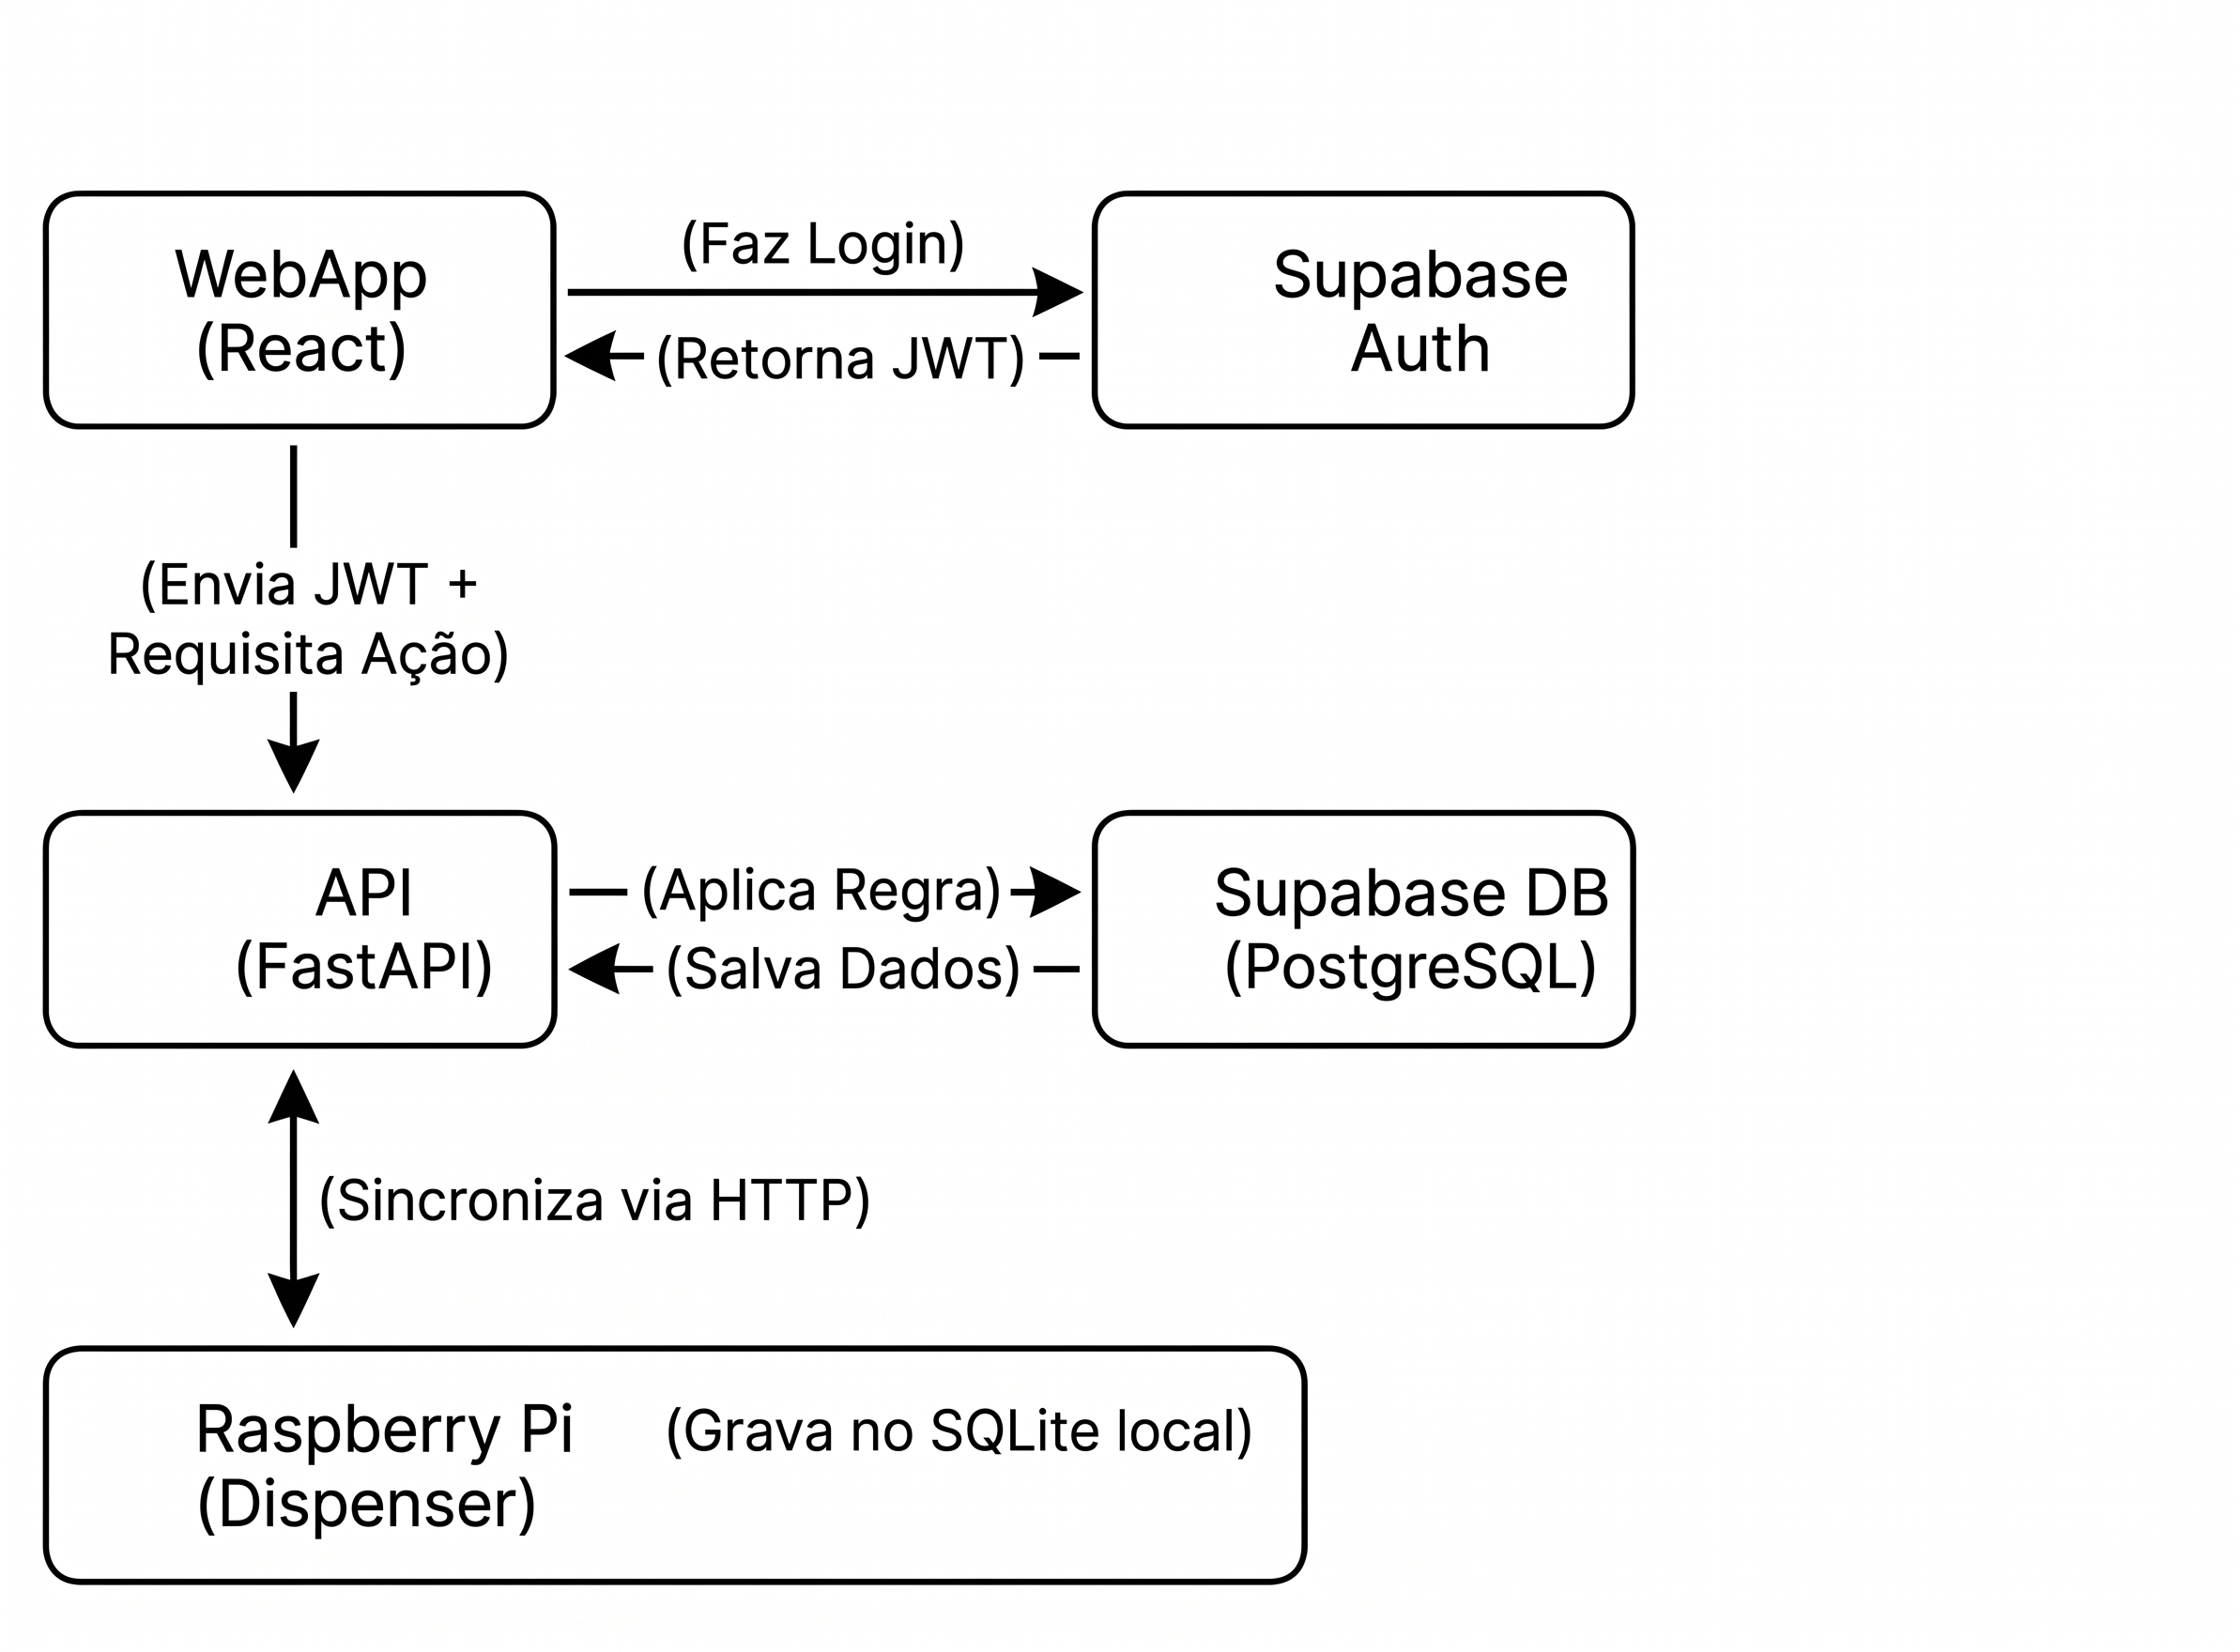
\includegraphics[width=0.82\textwidth,height=0.55\textheight,keepaspectratio]{Figuras/Artigo/arquitetura_artigo.png}
\fonte{Artigo e Anexo A, versão 2, material da equipe \cite{DC_ARTIGO}.}\end{figure}
\section{Arquitetura física e elétrica}
A ligação funcional possui quatro vias: +5 V, GND, SDA e SCL. Há um único SDA e um único SCL compartilhados; o intermediário os encaminha no mesmo nó aos submódulos e ao próximo andar, sem recriar outro barramento em GPIO diferentes. A Raspberry Pi é o controlador pretendido. A posição física dos contatos deve ser conferida por continuidade e não pela ordem de uma lista textual. \cite{DC_CIRCUITOS}
\section{Identidade, posição e conteúdo}
Endereço lógico, identidade de placa, posição física e medicamento são associações distintas. Mover um submódulo exige conferir e registrar a associação correspondente; um endereço não identifica automaticamente o conteúdo ou o novo local. O contrato posterior descreve instâncias e endereços derivados, mas a configuração realmente instalada deve ser comprovada por manifesto e leitura das placas. \cite{DC_COMPILADO}
\section{Evolução e divergências documentais}
O pré-relatório descreve Arduino Nano, conectores de cinco vias e fonte de 5 A; o mapa de setembro descreve ESP32, quatro vias e fonte prevista de 10 A. O artigo também preserva uma proposta de agente com Copilot Studio, enquanto a documentação de novembro relata Foundry e MCP. Esses registros pertencem a momentos e alcances diferentes; não são combinados em um circuito ou implantação supostamente únicos. \cite{DC_PREREL,DC_CIRCUITOS,DC_FOUNDRY}
\pendencia{ARQ01}{A autora enviará o subspace de arquitetura. Incorporar o diagrama da configuração final e confrontá-lo com esquema, versões e montagem real; não substituir o material prometido por inferência.}
\pendencia{ARQ02}{Fornecer esquema da montagem pós-reparos, orientação de cada pogo, continuidade e fotografias identificadas. O mapa funcional disponível não comprova ordem física nem estado atual de todos os módulos.}
\section{Estado relatado e restrições}
O registro de 12/11/2026 relata Raspberry Pi conectada, runtime 0.7.12, INT-01 0.3.1 e SUB-01 0.6.1 comunicando. Ao mesmo tempo informa ausência de RTC funcional, agenda automática desligada, \texttt{hardware\_ready=false} e necessidade de reconciliação do motor. Trata-se de uma fotografia documental datada, não de uma verificação executada nesta revisão nem de aceite final. \cite{DC_ANALISE}
\pendencia{ARQ04}{Confirmar a configuração na data de fechamento: hashes, versões, boot IDs, módulos montados, provisionamento e pré-condições de operação. Registrar RTC, agenda e comissionamento com evidências primárias.}

% Revisão consolidada: 25/11/2026. Não antecipa resultados finais.
\chapter{Desenvolvimento mecânico}
\section{Estrutura e princípio de dispensação}
O conjunto organiza a central, os intermediários e os submódulos removíveis. Em vez de compartimentos abastecidos por horário, cada reservatório é associado a um medicamento, e o disco busca separar a quantidade requerida. O material descreve reservatório, disco de cavidades, placa de apoio, acoplamento, trajeto de queda e recipiente coletor. Isso caracteriza a concepção; desempenho e limites por comprimido dependem de ensaio. \cite{DC_PREREL,DC_COMPILADO}
\section{Disco, inclinação e sequência funcional}
Adota-se 35\ensuremath{^{\circ}} como inclinação de projeto, conforme a decisão da autora e o pré-relatório. Não se trata de medida do conjunto impresso. O disco documentado tem cinco cavidades e é acionado pelo motor de passo. Capturar, transportar, liberar e reler a cavidade são etapas distintas. Não se assume que um avanço de uma cavidade correspondeu a uma unidade liberada. \cite{DC_PREREL,DC_COMPILADO}
\pendencia{MEC01}{Inserir CAD e desenho técnico finais, revisão, cotas e relação das peças fabricadas com o modelo. A inclinação adotada é 35\ensuremath{^{\circ}}; fornecer a evidência de fabricação e a medição do conjunto montado.}
\section{Dimensões recuperadas do modelo V75}
O compilado registra medidas extraídas do modelo digital V75. Elas ajudam a identificar peças e pontos críticos, mas não são medições físicas nem prova de correspondência com a versão escolhida. O V75 indica inclinação de 30\ensuremath{^{\circ}}, divergente dos 35\ensuremath{^{\circ}} adotados nesta revisão. Portanto, esses valores permanecem identificados como referência geométrica histórica. \cite{DC_COMPILADO}

{\small\setlength{\tabcolsep}{3pt}\begin{longtable}{p{0.25\textwidth}p{0.32\textwidth}p{0.31\textwidth}}\caption{Medidas documentais do V75, não verificadas na peça fabricada}\label{tab:07-1}\\
\hline
\textbf{Referência no V75} & \textbf{Valor documental} & \textbf{Limitação}\\\hline
\endfirsthead\hline
\textbf{Referência no V75} & \textbf{Valor documental} & \textbf{Limitação}\\\hline
\endhead
Disco & 57,3 mm de diâmetro; placa de 6,0 mm & Modelo digital; confirmar peça.\\\hline
Cavidades & Cinco furos de 11,0 mm; círculo de 39,6 mm & Confirmar geometria e medicamento compatível.\\\hline
Folga disco--reservatório & 0,72 mm na direção do eixo & Não medida após impressão.\\\hline
Canal vertical central & 30 mm & Não utilizar 60 mm de outro conceito.\\\hline
Copo coletor & 38,0 mm externos; parede aproximada de 1,5 mm; altura 34 mm & Confirmar se é o coletor instalado.\\\hline
Inclinação da referência & 30\ensuremath{^{\circ}} no V75; 35\ensuremath{^{\circ}} adotados para o projeto & Revisão CAD e medida física pendentes.\\\hline
\end{longtable}}{\small\noindent Fonte: Compilado da equipe, medidas recuperadas do modelo V75.\par}


\pendencia{MEC03}{Conferir as dimensões da peça fabricada com instrumento, revisão e incerteza apropriados. Medir disco, cavidades, folgas, aberturas, oscilação e trajeto até o coletor. Não converter cotas do V75 em valores medidos do protótipo.}
\section{Modelos apresentados no artigo}
As figuras permitem identificar o conceito mecânico e as partes do dosador no artigo. Não possuem, por si, identificação suficiente de revisão, material ou parâmetros de impressão; tampouco comprovam a inclinação da peça final. \cite{DC_ARTIGO}
\begin{figure}[htbp]\centering
\caption{Representação do reservatório e do disco no artigo, utilizada como referência conceitual.}
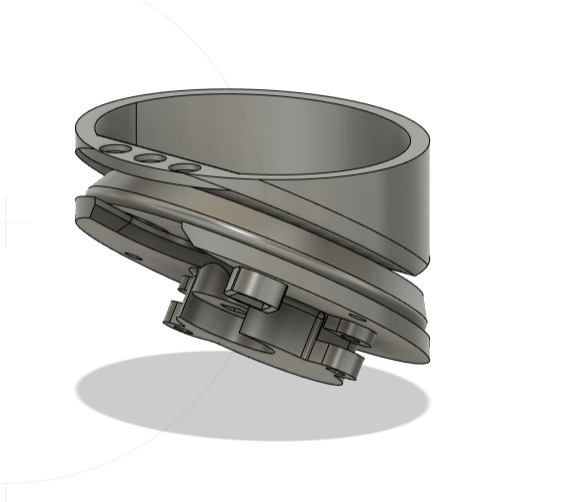
\includegraphics[width=0.82\textwidth,height=0.55\textheight,keepaspectratio]{Figuras/Artigo/cad_funil_artigo.jpeg}
\fonte{Artigo e Anexo A, versão 2, material da equipe \cite{DC_ARTIGO}.}\end{figure}
\begin{figure}[htbp]\centering
\caption{Vista inferior do componente dosador apresentada no artigo.}
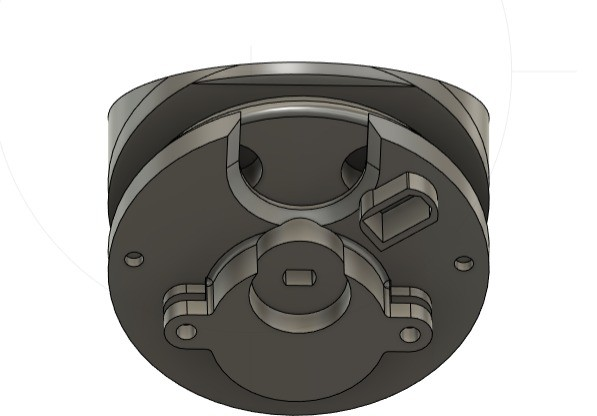
\includegraphics[width=0.82\textwidth,height=0.55\textheight,keepaspectratio]{Figuras/Artigo/cad_modulo_artigo.jpeg}
\fonte{Artigo e Anexo A, versão 2, material da equipe \cite{DC_ARTIGO}.}\end{figure}
A representação do conjunto completo no artigo é apresentada a seguir. Trata-se de modelo CAD, não de fotografia do protótipo montado nem de comprovação de ensaio. \cite{DC_ARTIGO}
\begin{figure}[htbp]\centering
\caption{Representação CAD do conjunto completo apresentada no artigo.}
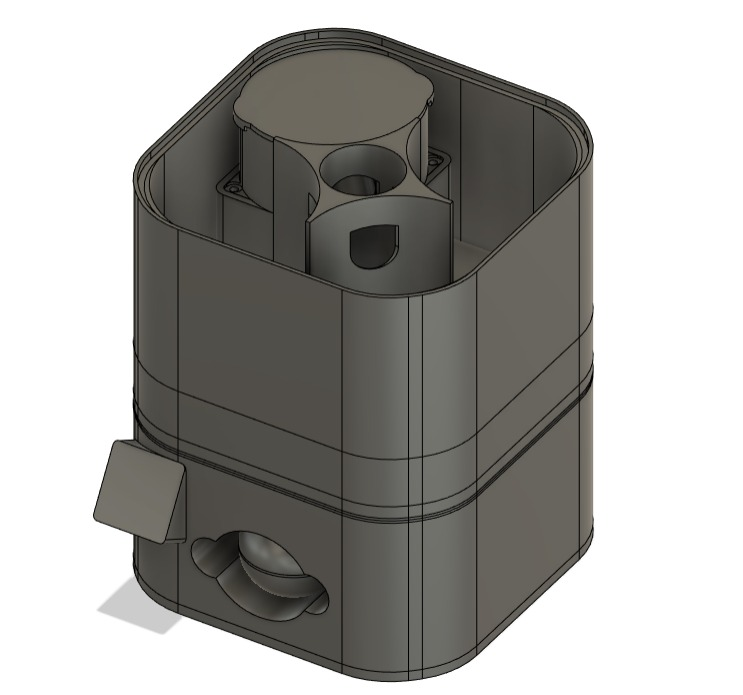
\includegraphics[width=0.65\textwidth,height=0.48\textheight,keepaspectratio]{Figuras/Artigo/conjunto_completo_artigo.jpeg}
\fonte{Artigo e Anexo A, versão 2, material da equipe \cite{DC_ARTIGO}.}
\end{figure}

\section{Materiais, impressão e fixação}
As listas fornecidas preveem PLA branco, parafusos M3 e ímãs. Material comprado não equivale a material usado em cada peça. O compilado descreve alojamentos e folgas no V75 e recomenda registrar parâmetros por componente. Não foi fornecido nesta rodada o material complementar prometido com o inventário final instalado. \cite{DC_LISTA,DC_PROPOSTA,DC_COMPILADO}
\pendencia{MEC04}{Inserir a ficha de fabricação por peça: material/marca/lote, impressora, fatiador, revisão, bico, temperaturas, camada, perímetros, preenchimento, orientação, suportes, tempo e massa. A lista de compra já foi recebida; falta a fabricação efetiva.}
\pendencia{MEC05}{Completar a lista técnica instalada: parafusos por posição, ímãs e polaridade, acoplamentos, pogo, retenção, ajustes e eventual uso de adesivo. Incorporar o material complementar a ser fornecido pela autora.}
\section{Montagem, manutenção e limpeza}
A remoção do submódulo é um requisito de projeto, mas demanda verificar retenção, alinhamento e continuidade durante ciclos de encaixe. O funcionamento com medicamentos exige também conhecer o acabamento das superfícies, o procedimento de limpeza e a possibilidade de retenção de resíduos. Não há base para declarar adequação sanitária ou durabilidade sem esses registros. \cite{DC_COMPILADO}
\pendencia{MEC06-FOTO1}{INSERIR FOTO: vista geral do protótipo físico final, identificando revisão, módulos presentes e data. A figura CAD do artigo não substitui a fotografia.}
\pendencia{MEC06-FOTO2}{INSERIR FOTOS: disco, cavidades, reservatório, placa de apoio, saída, coletor, fixação do motor e contatos. Incluir escala e legenda, sem dados pessoais.}
\section{Verificações mecânicas pendentes}
\pendencia{MEC07}{Registrar massas, inclinação medida, atrito/ângulo de deslizamento, retenção desenergizada, folgas após impressão, desgaste e ciclos de encaixe. Para cada tipo de comprimido de teste, registrar captura simples/dupla, retenção, travamento, tentativas e falhas com denominador. Não há resultados finais fornecidos.}

\chapter{Desenvolvimento elétrico e eletrônico}\label{cap:eletrica}
A organização elétrica acompanha a divisão modular do aparelho. A central distribui alimentação e coordena o barramento; o intermediário controla a sinalização; e o submódulo reúne o acionamento e a leitura óptica. O projeto separa os ramais de potência de 5 V da lógica de 3,3 V e mantém referência de terra comum.

\section{Distribuição da alimentação}
Foi prevista uma fonte regulada de 5 V com capacidade nominal de 10 A. A distribuição utiliza ramais para a Raspberry Pi, o buzzer e a cadeia de módulos. No submódulo, a alimentação atende à ESP32 e à placa de acionamento do motor, enquanto o circuito óptico utiliza a referência de 3,3 V. A Figura~\ref{fig:distribuicao_alimentacao} apresenta a organização funcional. \cite{DC_CIRCUITOS}

\begin{figure}[htbp]
\centering
\caption{Distribuição funcional da alimentação de 5 V e da referência comum}\label{fig:distribuicao_alimentacao}
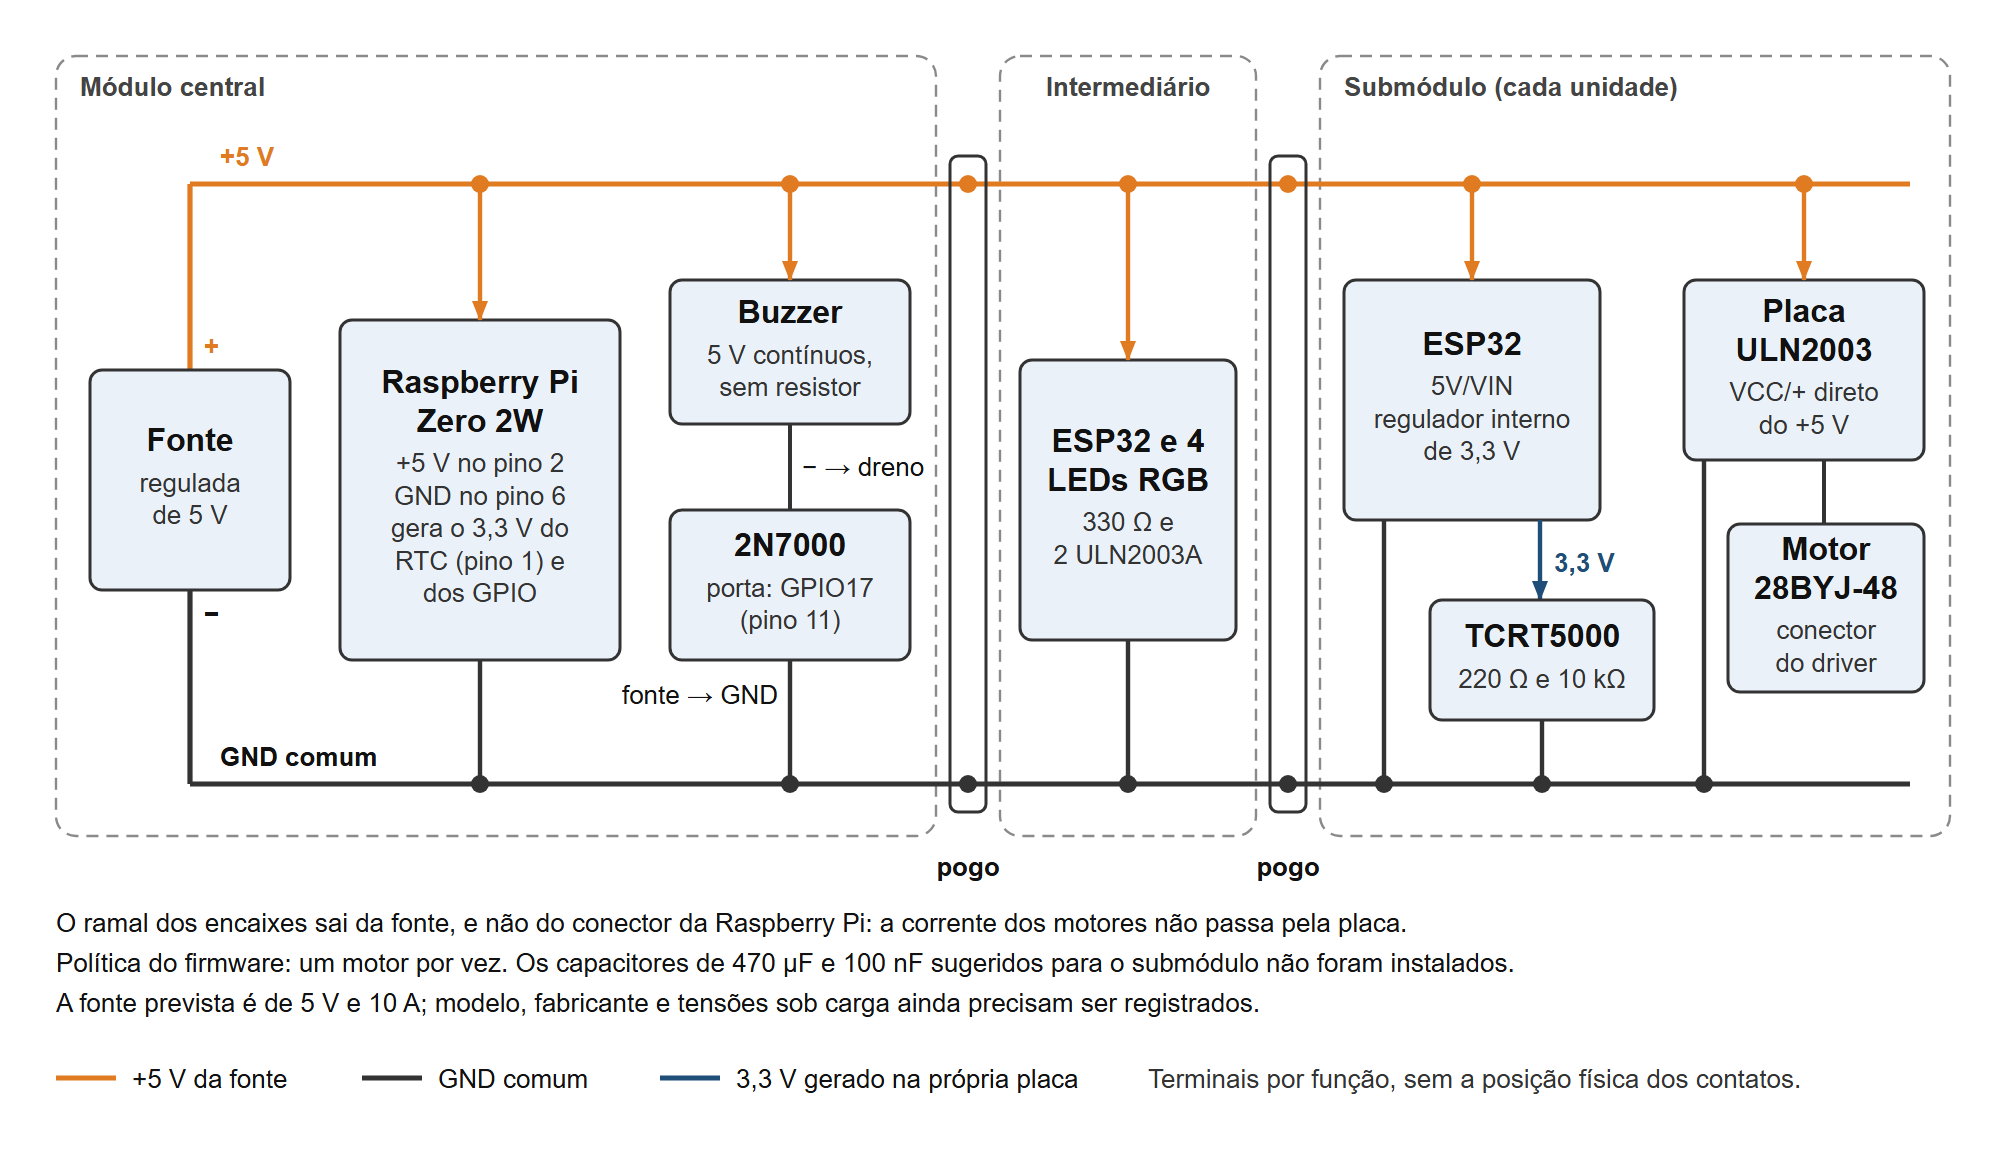
\includegraphics[width=0.98\textwidth,height=0.66\textheight,keepaspectratio]{Figuras/SharePoint/distribuicao_alimentacao.png}
\fonte{Elaboração dos autores (2026).}
\end{figure}


A corrente nominal da fonte não corresponde ao consumo do aparelho. A avaliação do fornecimento considera queda de tensão e corrente durante repouso, comunicação e atuação. O retorno comum também precisa manter referência adequada entre os sinais, evitando que o acionamento do motor comprometa as leituras e o barramento.

\section{Unidade central}
A Raspberry Pi Zero 2 W utiliza GPIO2 para SDA e GPIO3 para SCL, com lógica de 3,3 V. A central também reúne o módulo de relógio HW-084 com DS3231M, o buzzer e os sinais luminosos. Na coleta de 26 de novembro, o RTC não estava ativado no Linux; o tempo confiável dependia da rede. A presença de bateria compatível ainda precisava ser conferida. \cite{DC_VALIDACAO2026} A Figura~\ref{fig:circuito_central} apresenta as ligações por função. A interface de quatro vias deve ser identificada por continuidade, pois uma relação textual de sinais não determina sua ordem física no conector.

\begin{figure}[htbp]
\centering
\caption{Ligações funcionais da unidade central}\label{fig:circuito_central}
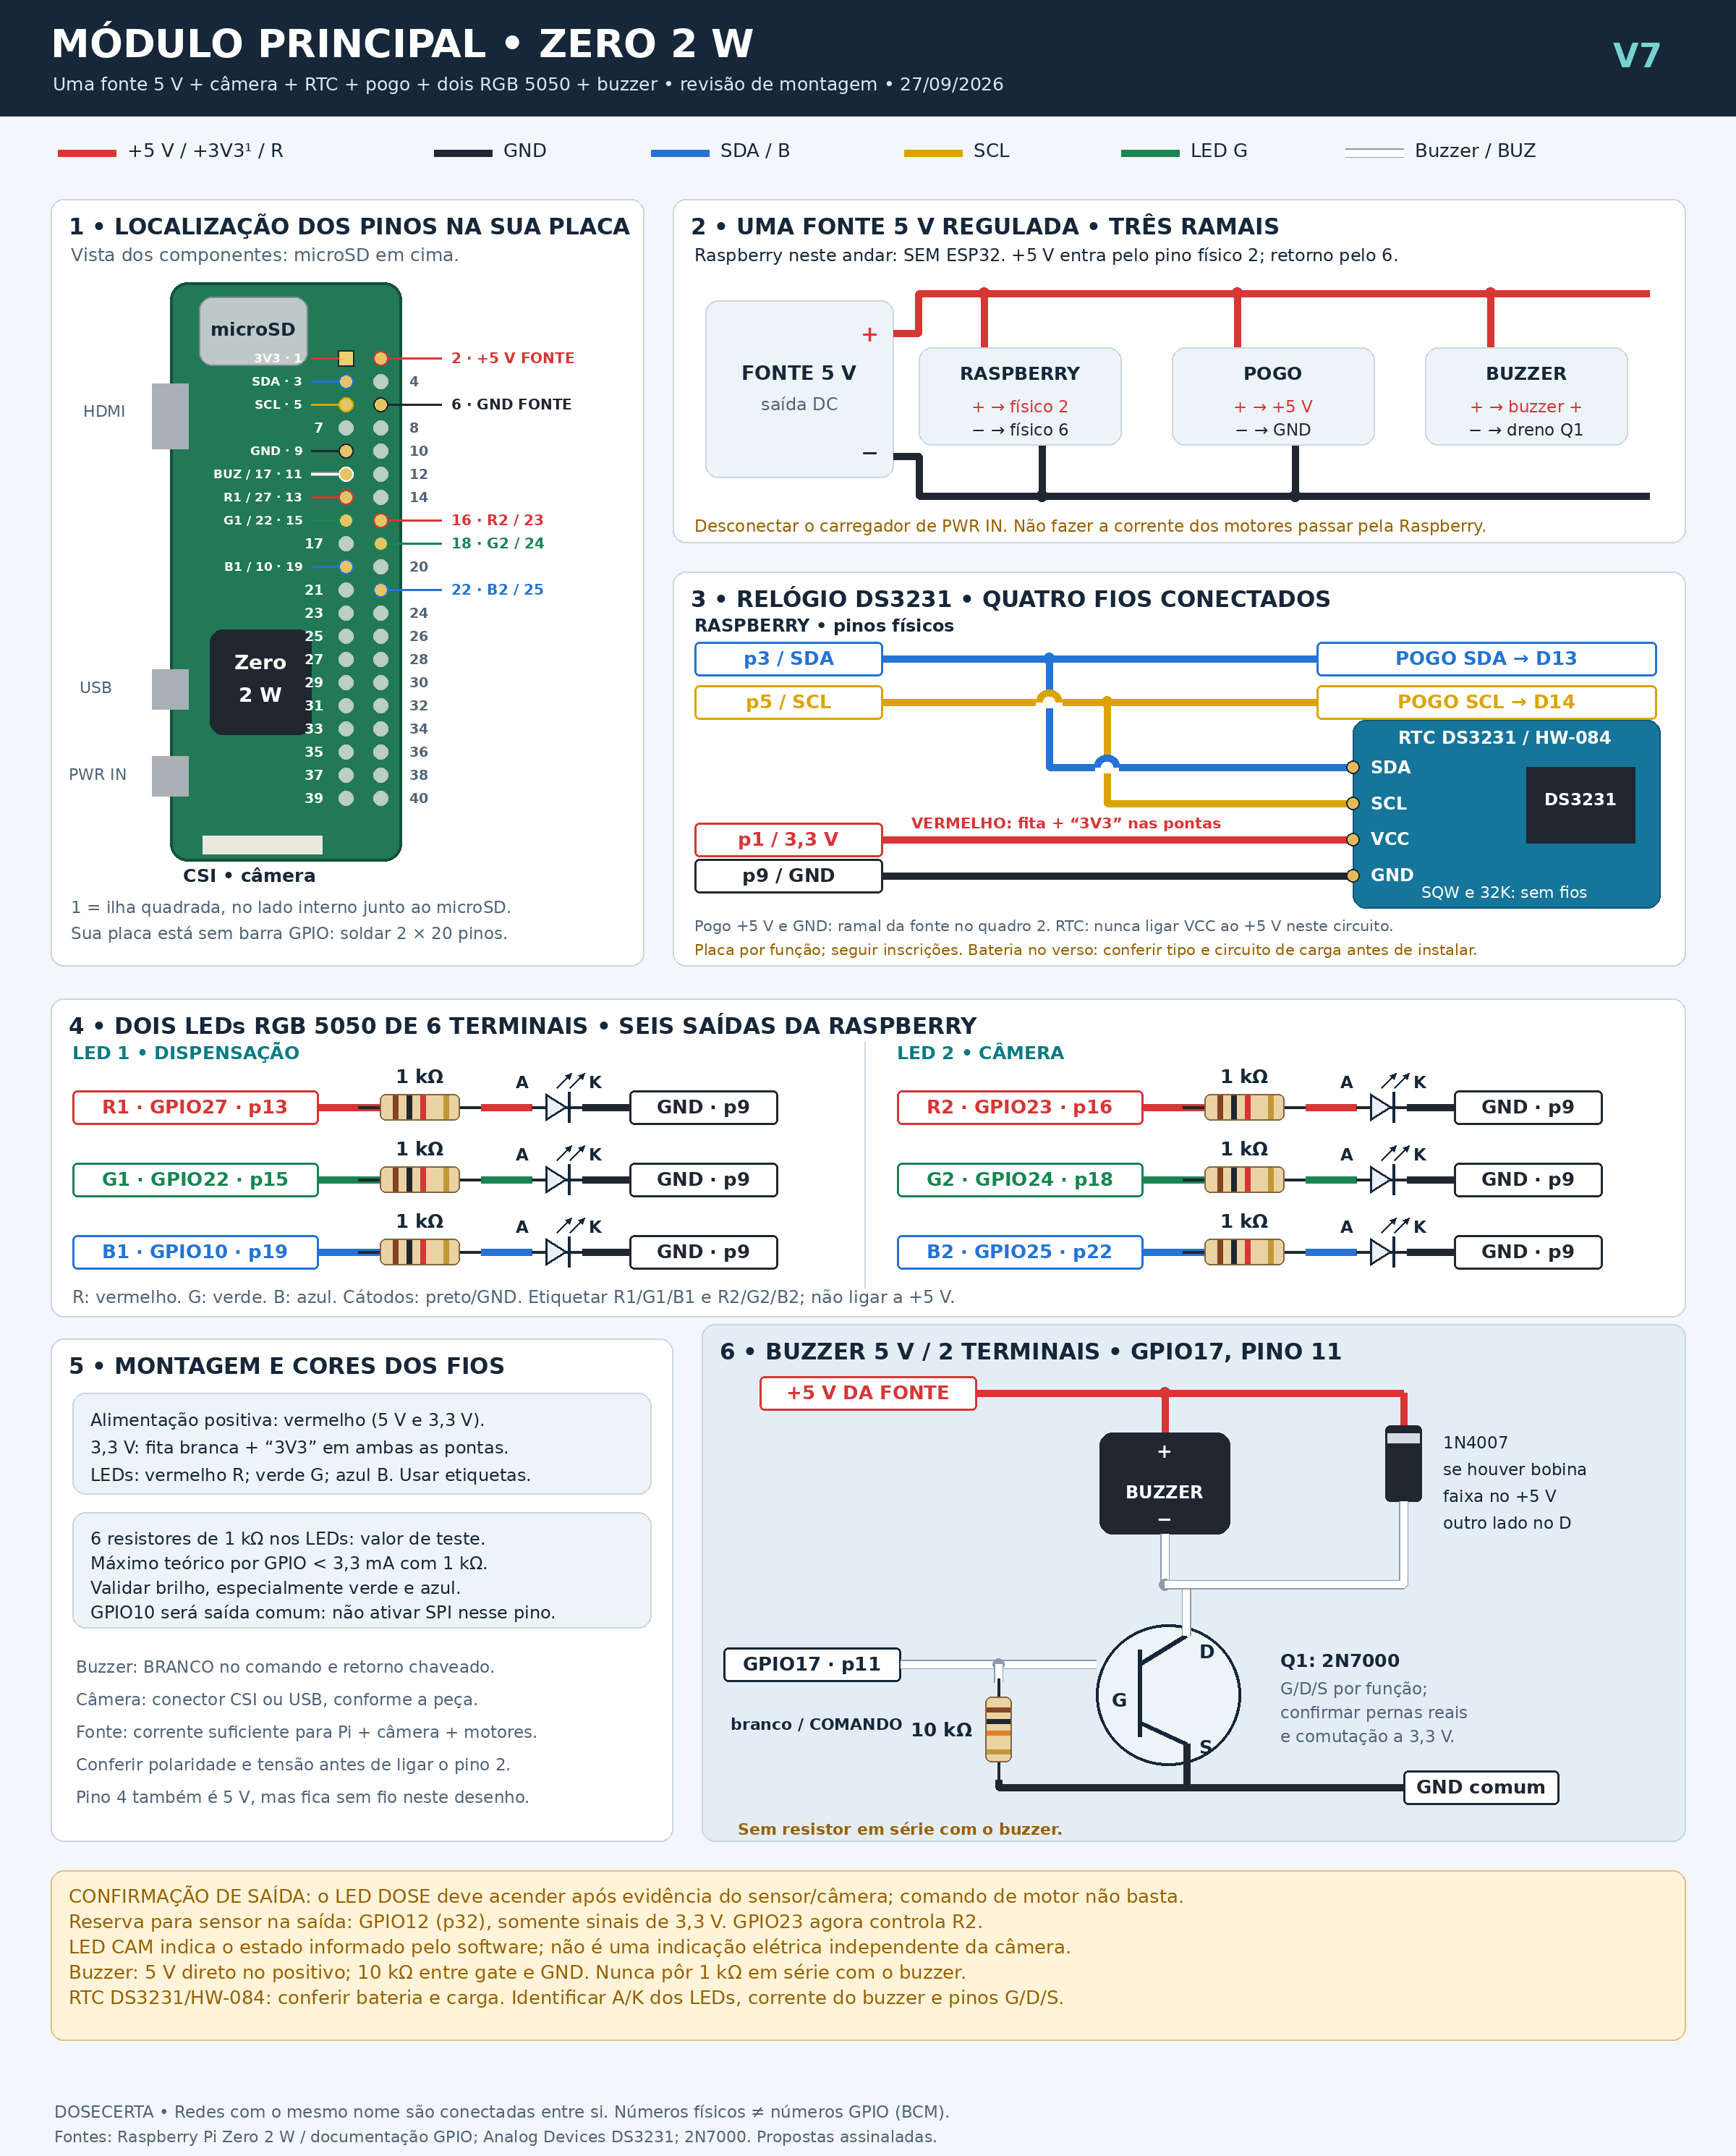
\includegraphics[width=0.98\textwidth,height=0.73\textheight,keepaspectratio]{Figuras/SharePoint/circuito_central.png}
\fonte{Elaboração dos autores (set. 2026). Distribuição funcional, sem definição da ordem física dos contatos.}
\end{figure}


O buzzer é alimentado pelo ramal de 5 V e chaveado pelo transistor 2N7000. O GPIO17 atua na porta, e o resistor de 10 k\ensuremath{\Omega} entre porta e fonte mantém a condição de desligamento. A Figura~\ref{fig:buzzer} detalha esse estágio. A identificação dos terminais e a condução com 3,3 V devem ser conferidas para o componente instalado.

\begin{figure}[htbp]
\centering
\caption{Estágio de acionamento do buzzer com transistor 2N7000}\label{fig:buzzer}
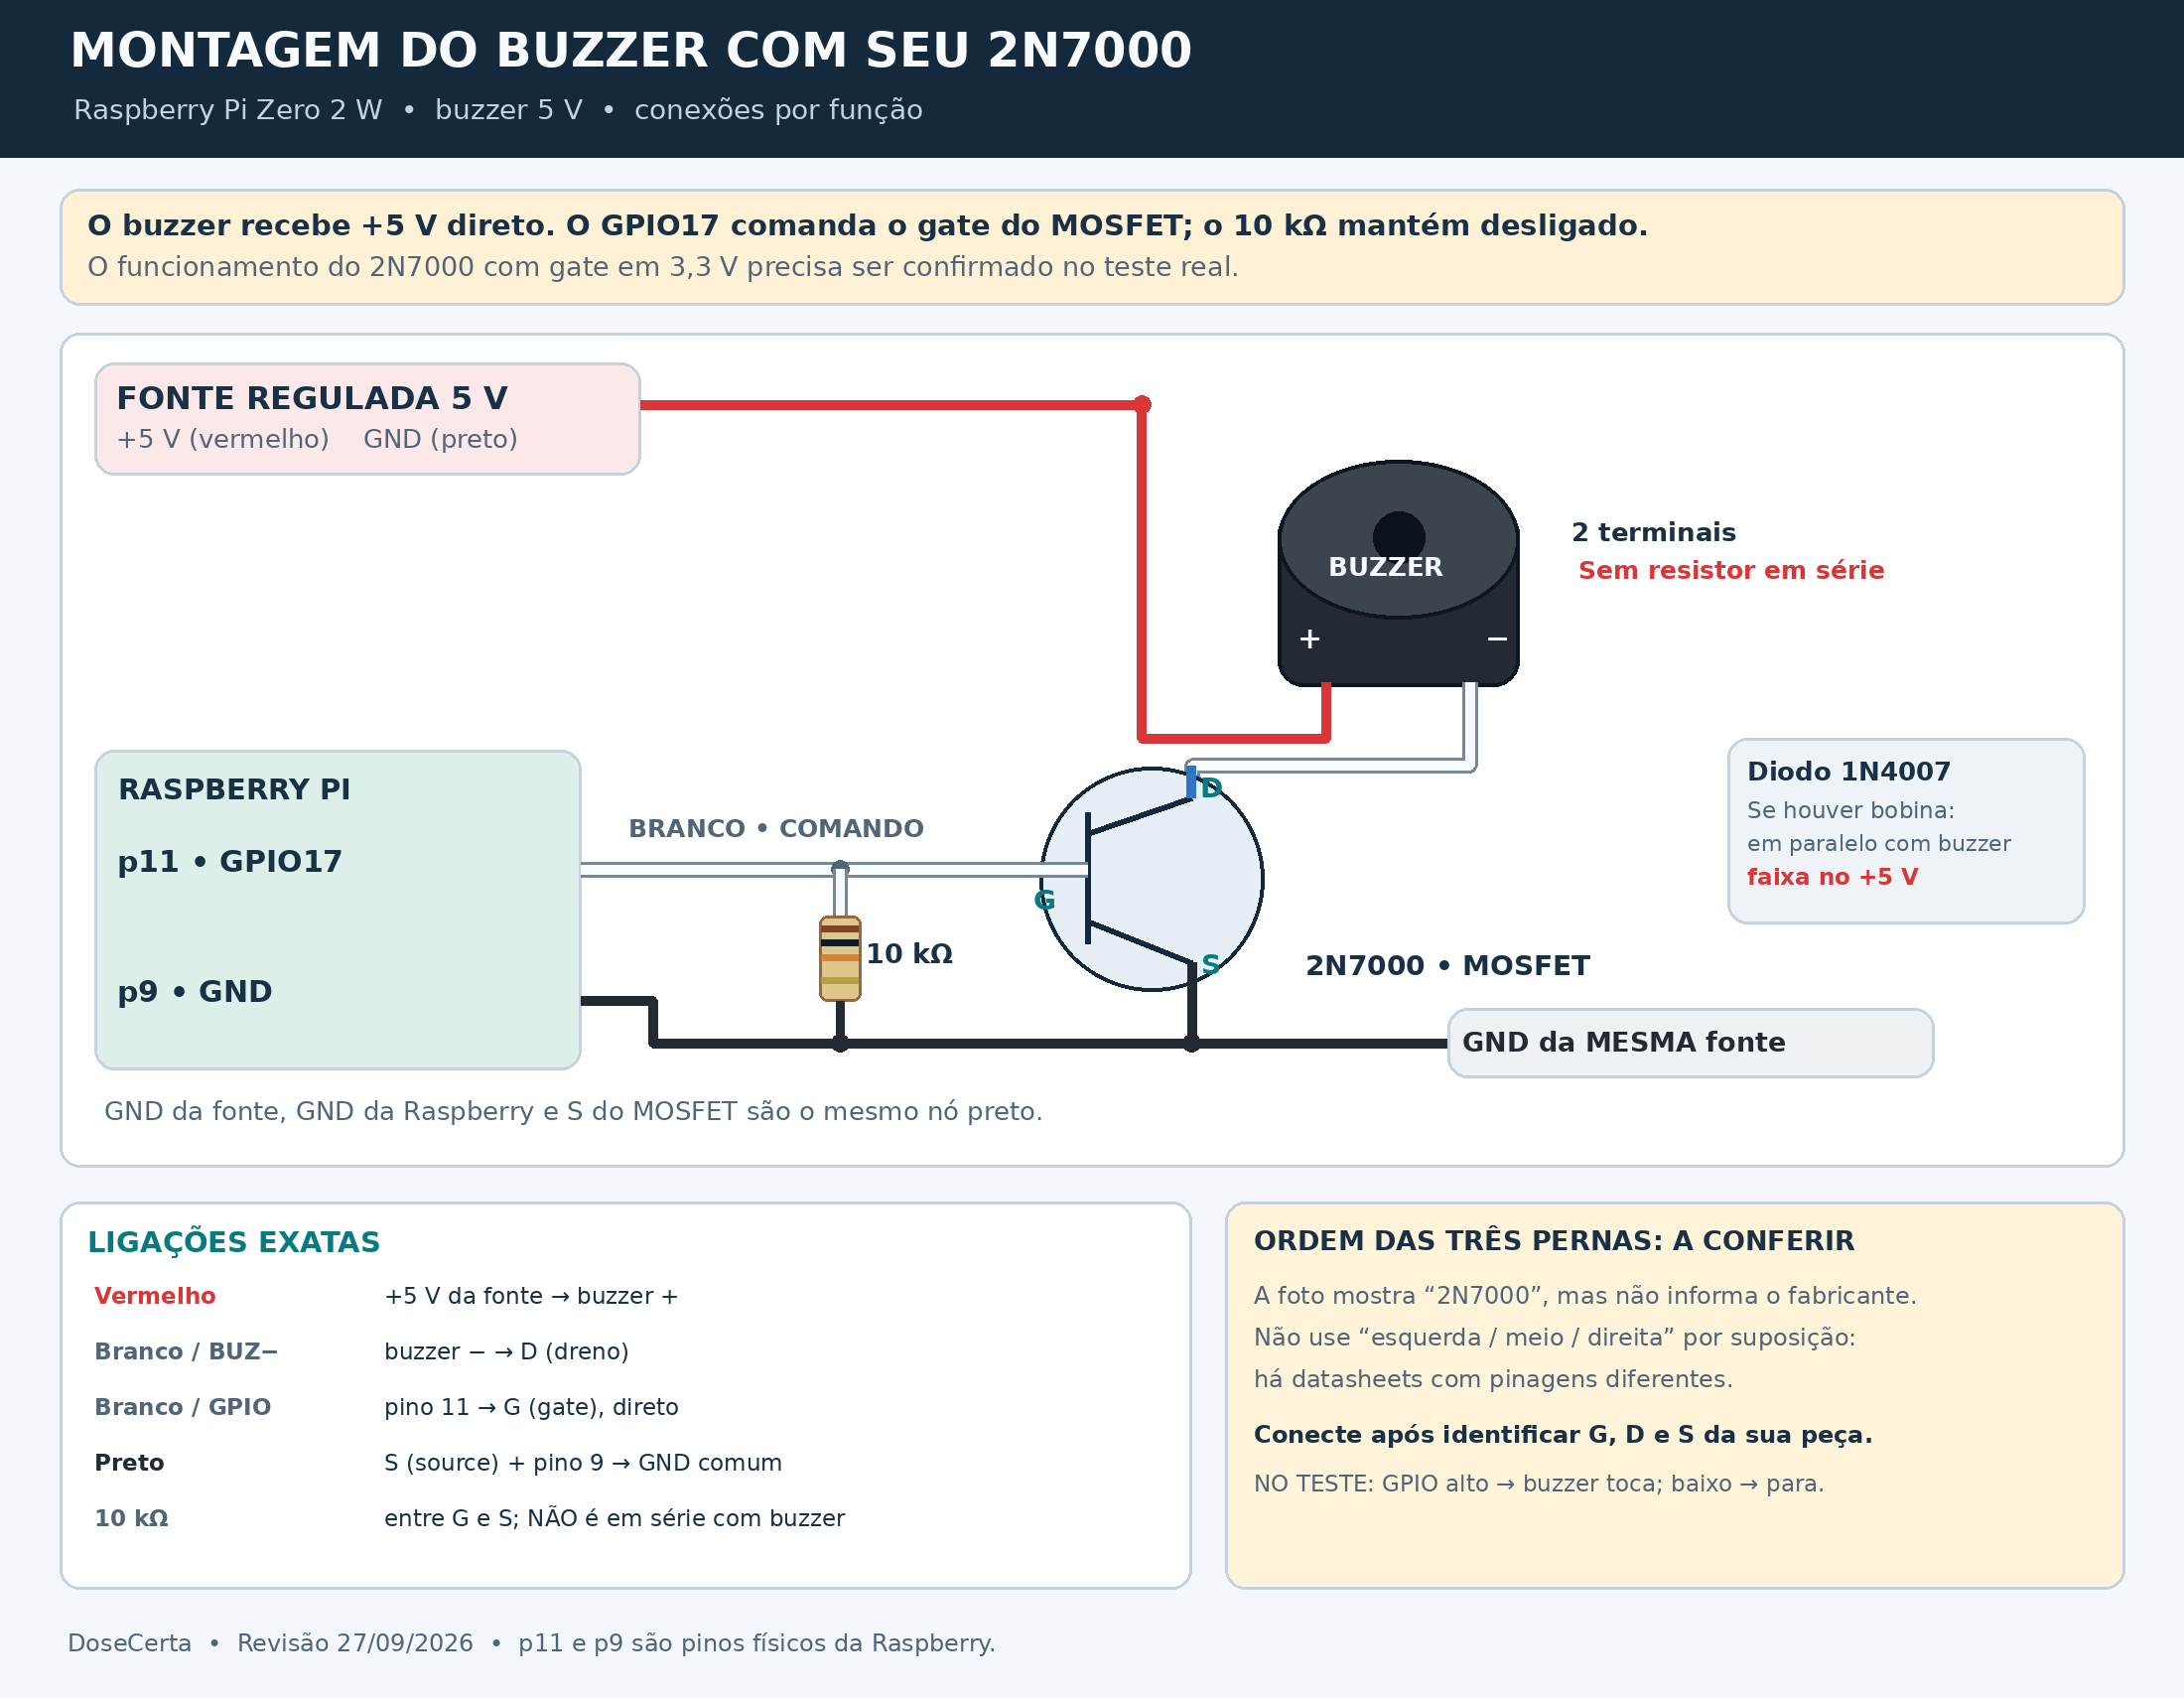
\includegraphics[width=0.91\textwidth,height=0.66\textheight,keepaspectratio]{Figuras/SharePoint/buzzer.png}
\fonte{Elaboração dos autores (set. 2026). Terminais e condição de acionamento dependem da peça utilizada.}
\end{figure}


\section{Submódulo dosador}
No submódulo, a ESP32 controla o 28BYJ-48 por meio da placa ULN2003 e lê o TCRT5000 no ADC1. Os sinais do motor utilizam GPIO27, GPIO26, GPIO25 e GPIO33, e a leitura óptica utiliza GPIO32. O barramento chega aos GPIO13 e GPIO14. A Figura~\ref{fig:circuito_submodulo} reúne essas ligações.

\begin{figure}[htbp]
\centering
\caption{Ligações funcionais do submódulo dosador}\label{fig:circuito_submodulo}
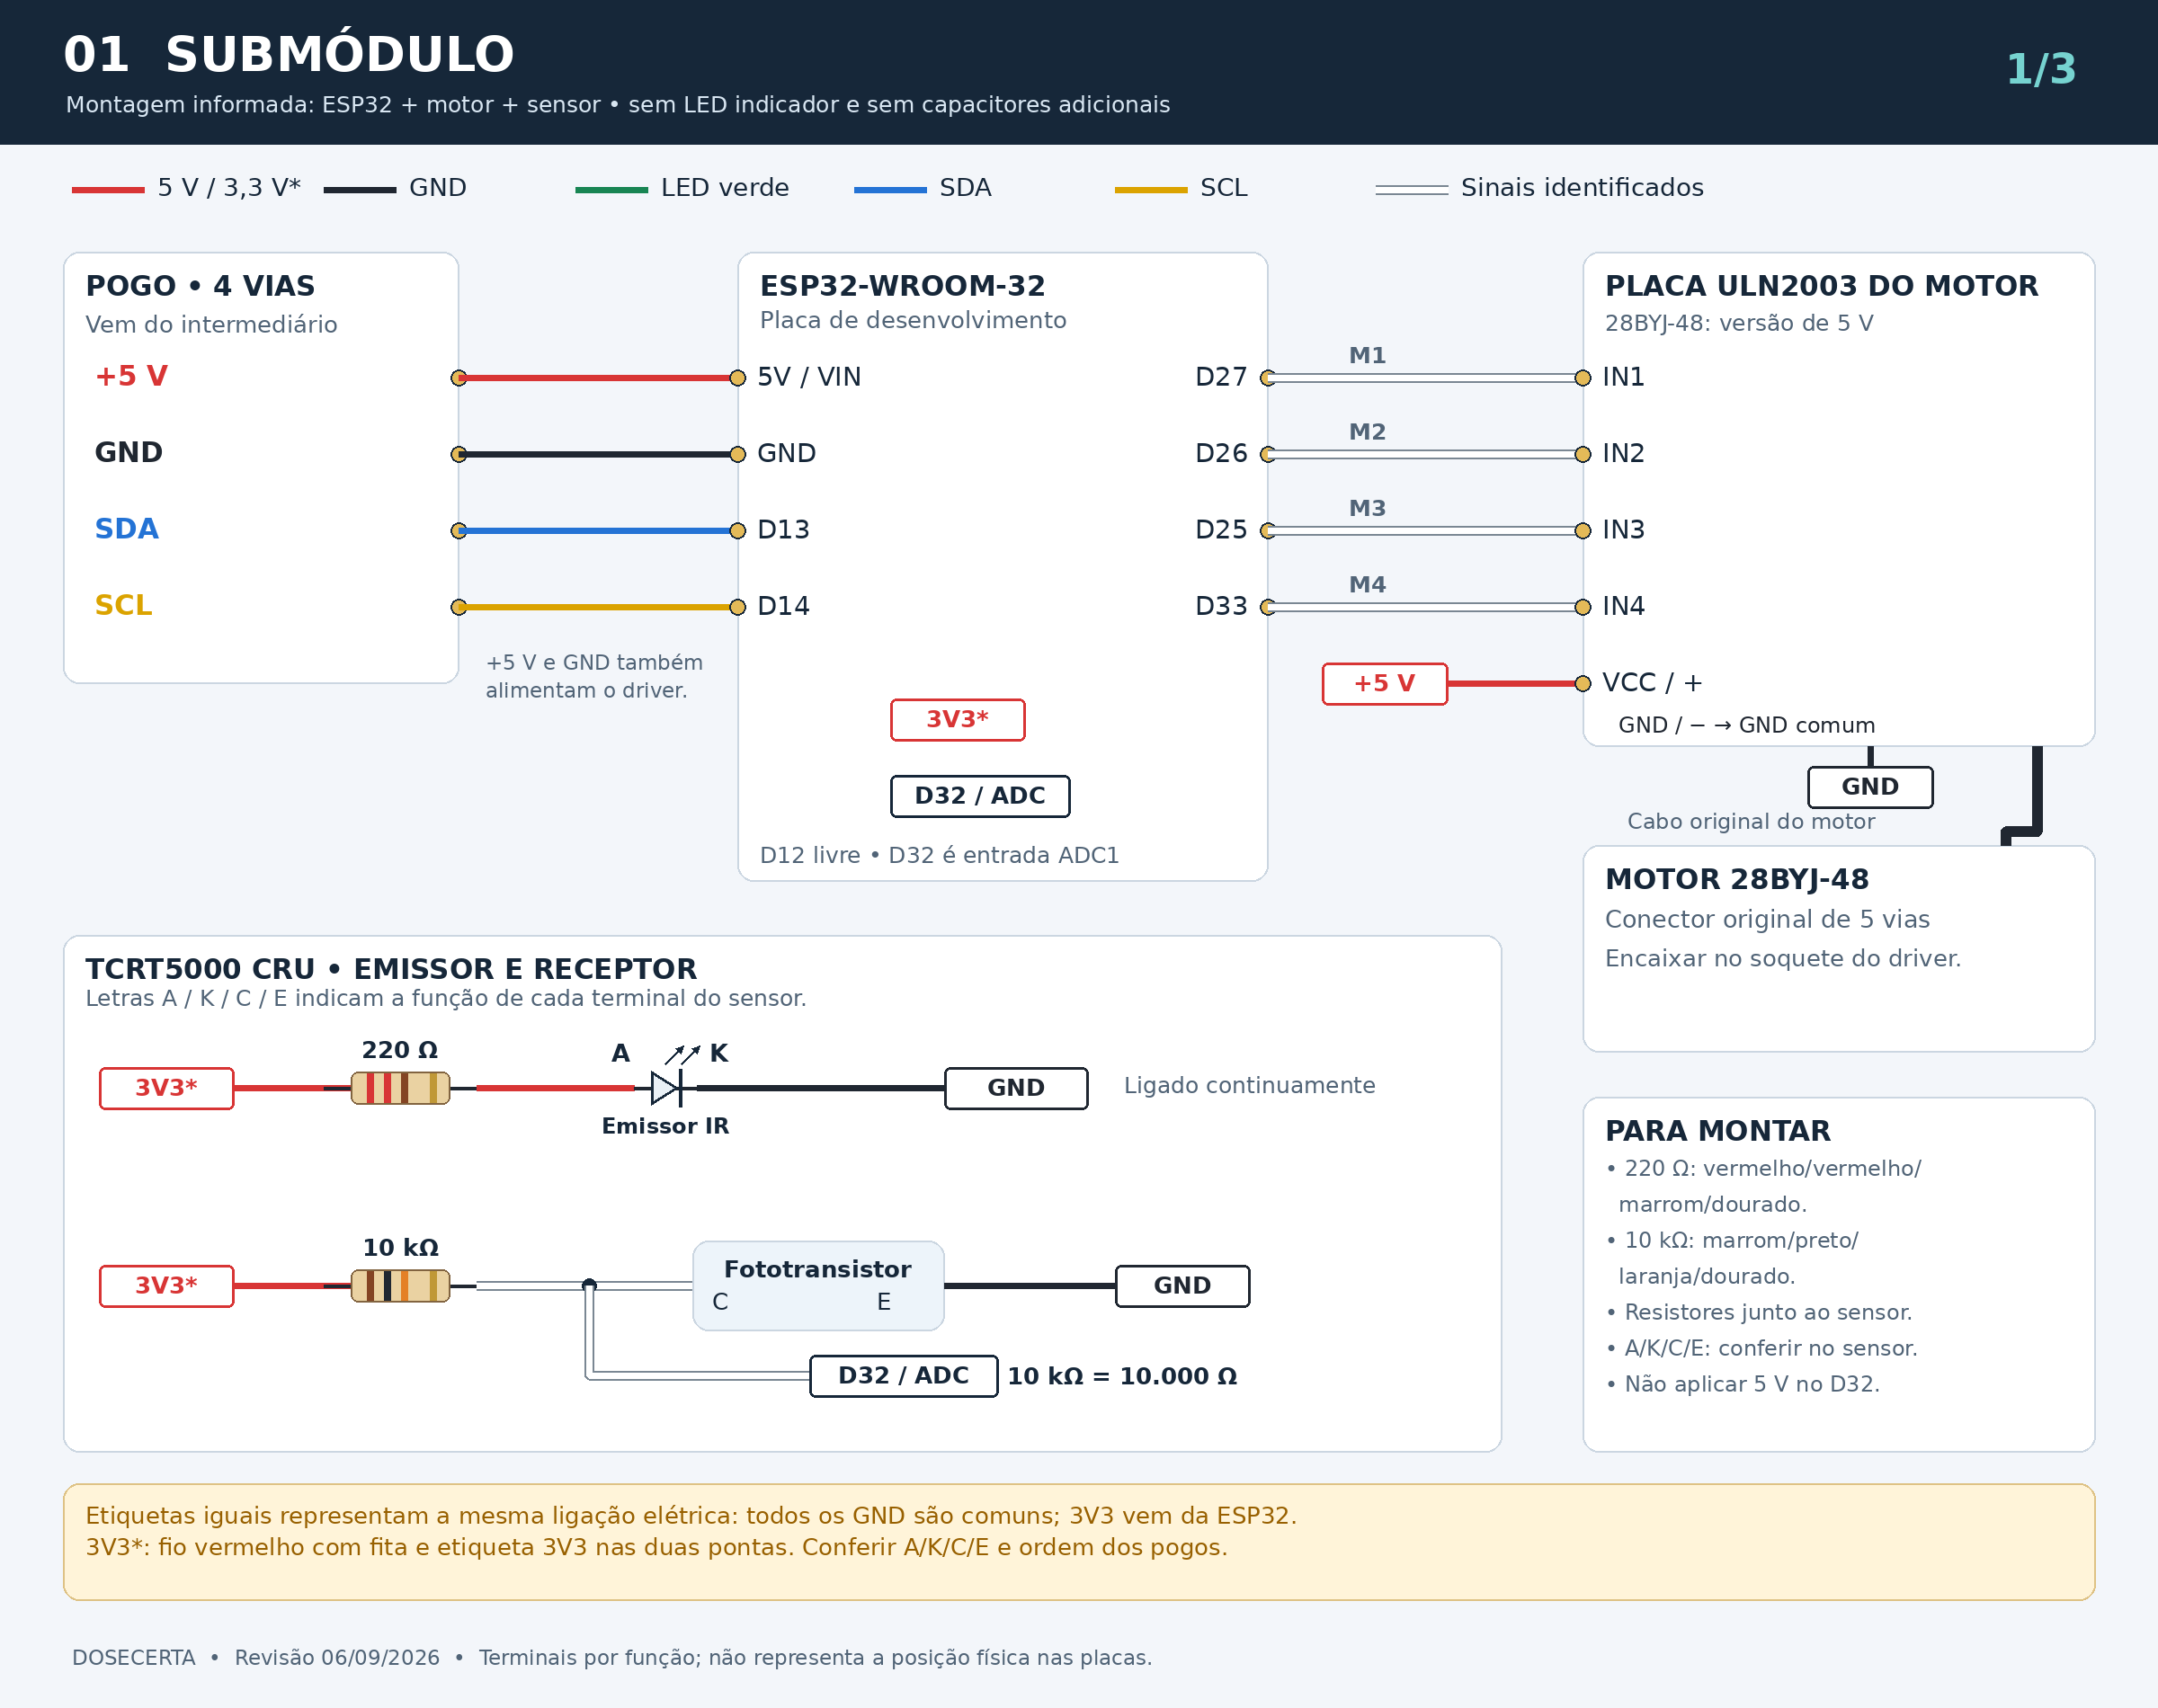
\includegraphics[width=0.98\textwidth,height=0.70\textheight,keepaspectratio]{Figuras/SharePoint/circuito_submodulo.png}
\fonte{Elaboração dos autores (set. 2026). Prancha anterior às correções finais de bancada.}
\end{figure}


O emissor infravermelho utiliza resistor de 220\ensuremath{\Omega}; o fototransistor é lido com resistor de 10 k\ensuremath{\Omega} para 3,3 V. A leitura é interpretada em conjunto com o movimento e a calibração, não como um detector independente de ingestão. O acionamento do motor utiliza a alimentação de potência, sem retirar corrente das saídas lógicas do microcontrolador.

\section{Intermediário e sinalização}
O intermediário utiliza quatro LEDs RGB 5050, associados aos canais L1 a L4. Os sinais são chaveados por dois ULN2003A, com resistores de 330\ensuremath{\Omega} nos canais de cor. A Figura~\ref{fig:circuito_intermediario} apresenta a topologia funcional, e a Tabela~\ref{tab:eletrica-gpio} relaciona os GPIO. \cite{DC_CIRCUITOS}

\begin{figure}[htbp]
\centering
\caption{Ligações funcionais dos LEDs e dos drivers do intermediário}\label{fig:circuito_intermediario}
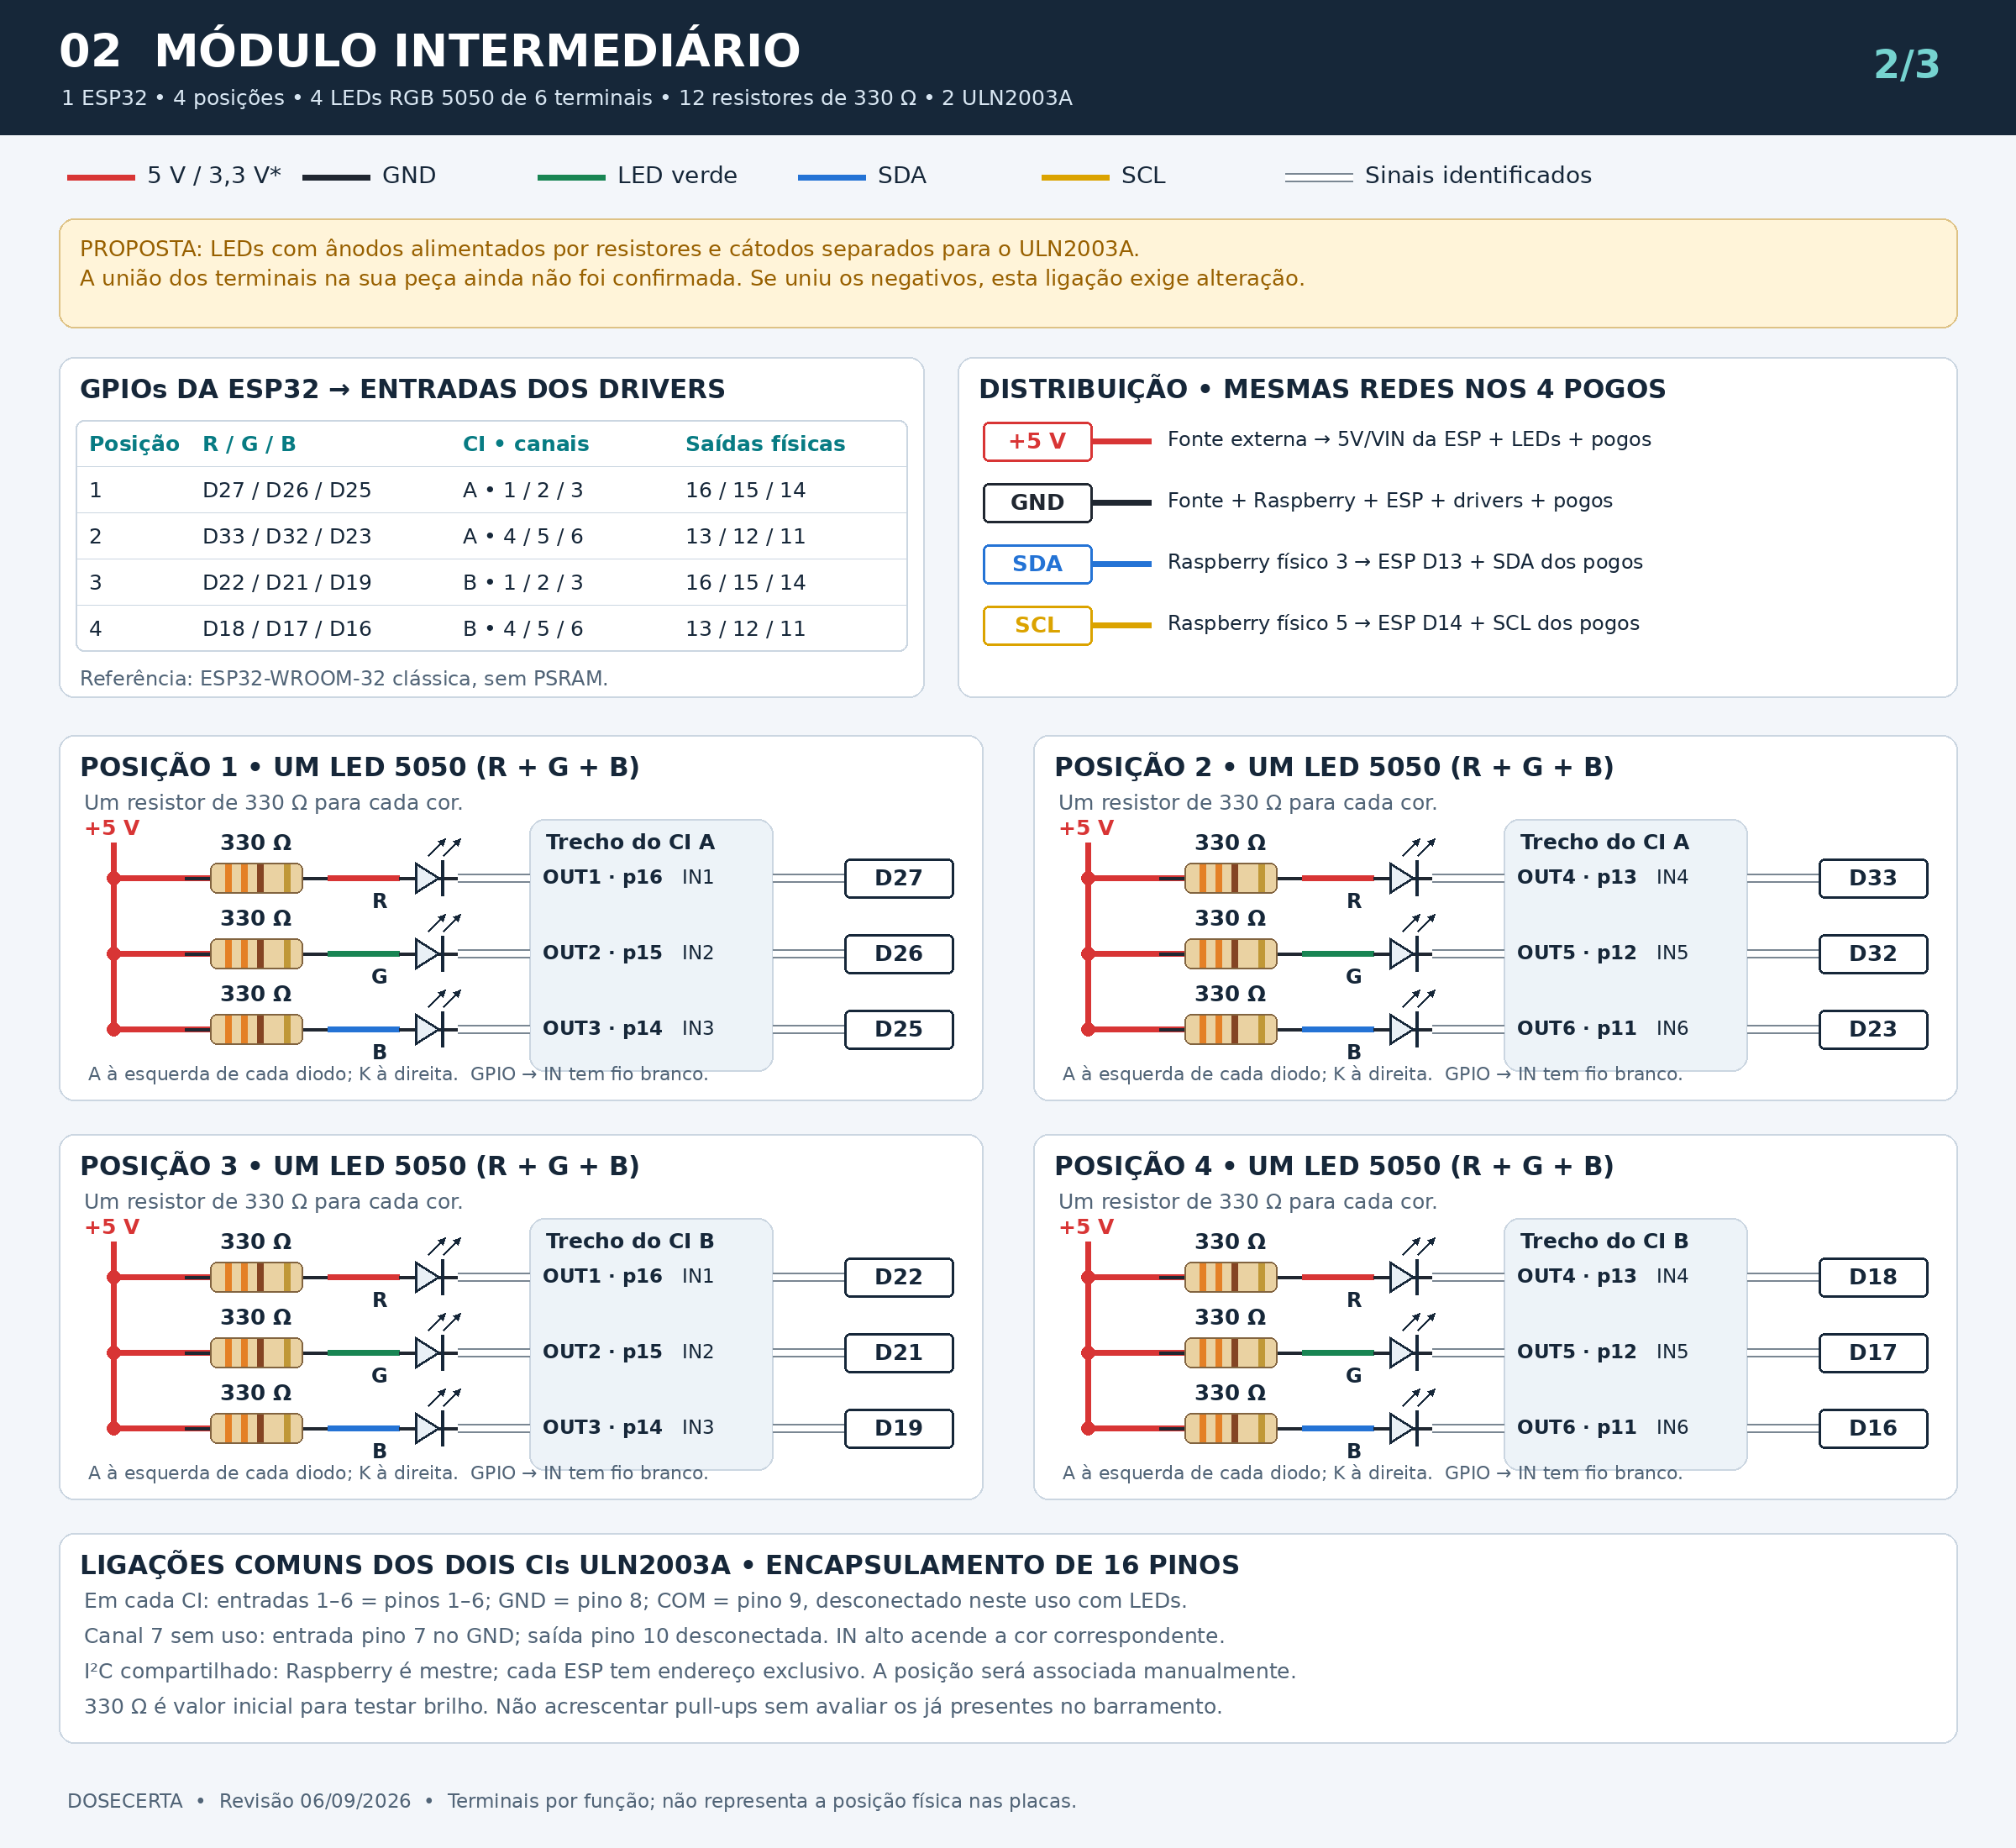
\includegraphics[width=0.98\textwidth,height=0.70\textheight,keepaspectratio]{Figuras/SharePoint/circuito_intermediario.png}
\fonte{Elaboração dos autores (set. 2026). Topologia a conferir na montagem final.}
\end{figure}


{\small\begin{longtable}{p{0.22\textwidth}p{0.22\textwidth}p{0.22\textwidth}p{0.22\textwidth}}
\caption{GPIO dos canais luminosos do intermediário}\label{tab:eletrica-gpio}\\
\hline\textbf{Canal} & \textbf{Vermelho} & \textbf{Verde} & \textbf{Azul}\\\hline\endfirsthead
\hline\textbf{Canal} & \textbf{Vermelho} & \textbf{Verde} & \textbf{Azul}\\\hline\endhead
L1 & 27 & 26 & 25\\\hline
L2 & 33 & 32 & 23\\\hline
L3 & 22 & 21 & 19\\\hline
L4 & 18 & 17 & 16\\\hline
\end{longtable}\noindent Fonte: projeto elétrico dos autores.\par}

A disposição dos encaixes e dos canais é mostrada na Figura~\ref{fig:encaixes_intermediario}. Cada posição fica entre dois LEDs, permitindo identificá-la pelo par adjacente. Assim, a confirmação visual de uma posição não depende de um LED instalado no submódulo.

\begin{figure}[htbp]
\centering
\caption{Disposição funcional dos encaixes e canais luminosos do intermediário}\label{fig:encaixes_intermediario}
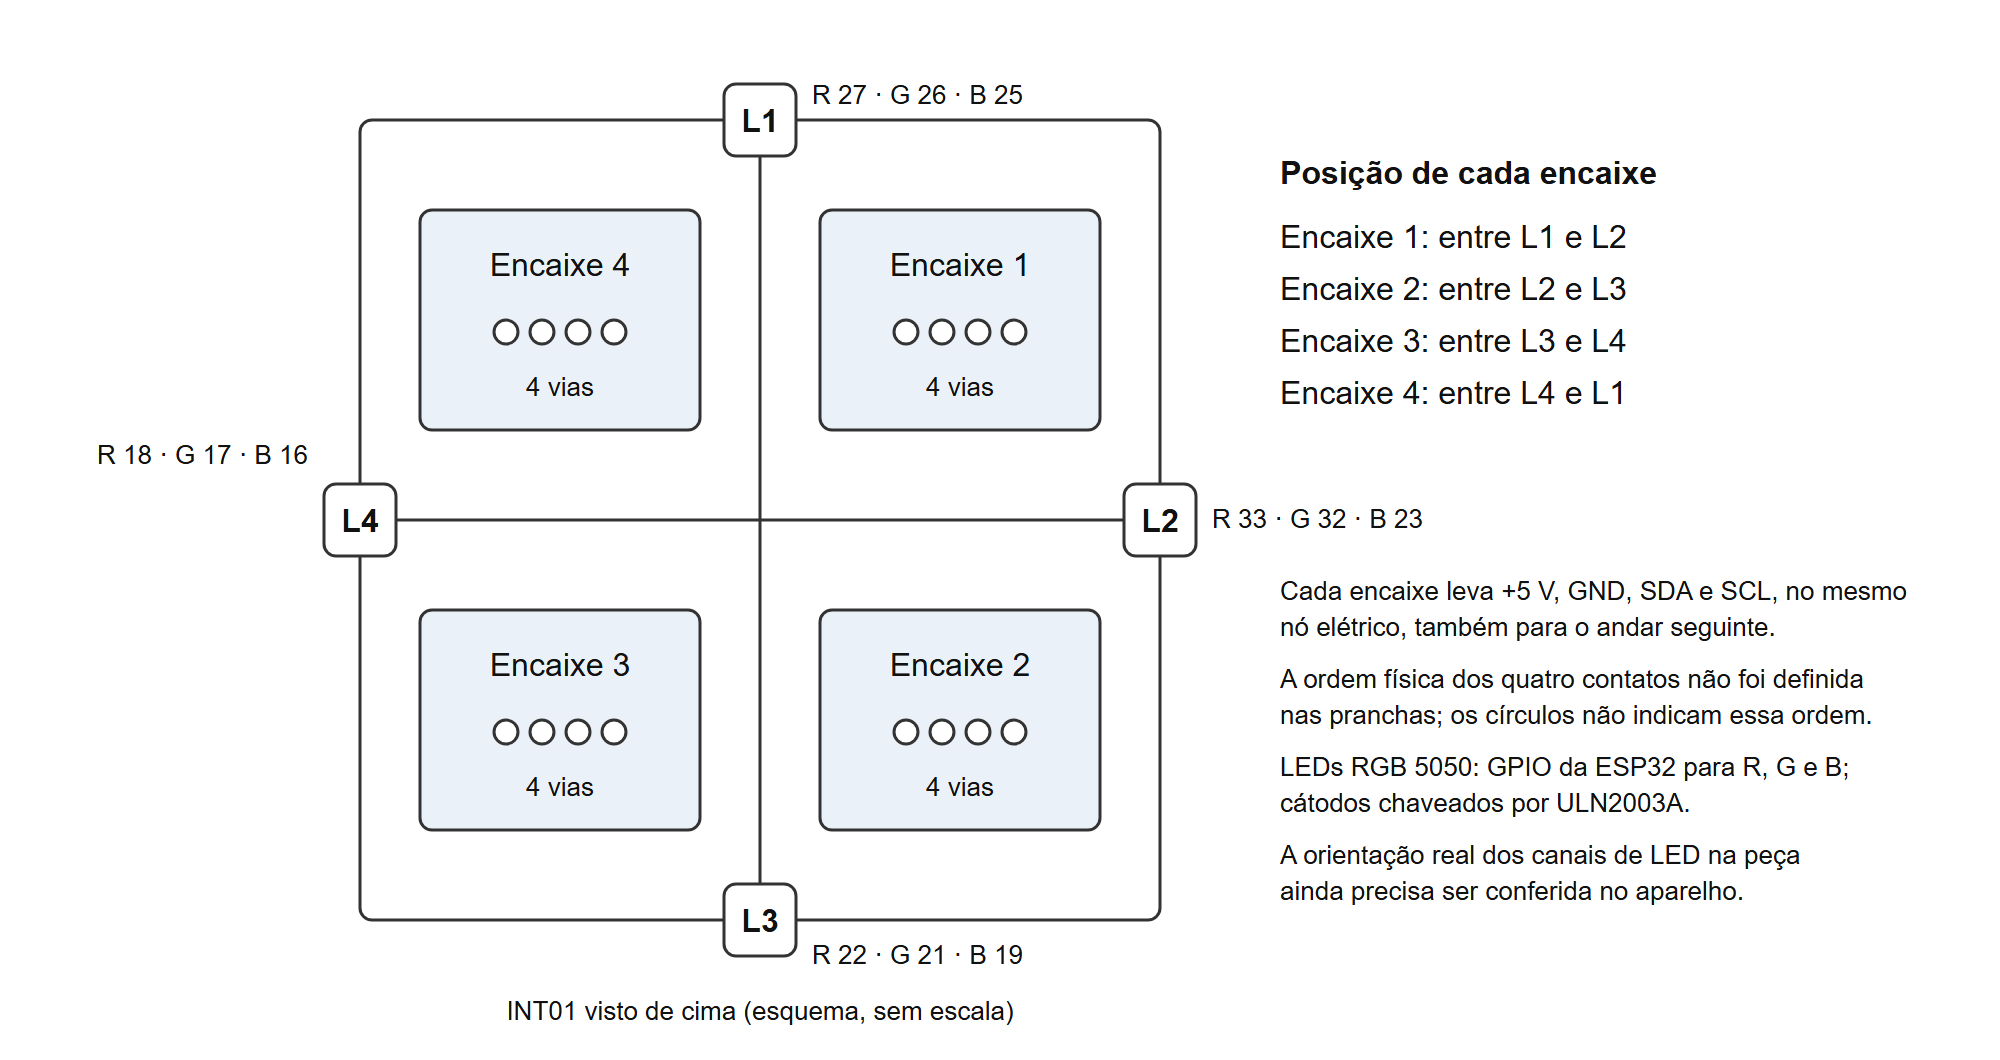
\includegraphics[width=0.98\textwidth,height=0.66\textheight,keepaspectratio]{Figuras/SharePoint/encaixes_intermediario.png}
\fonte{Elaboração dos autores (2026).}
\end{figure}


\section{Barramento, contatos e verificações}
As vias de alimentação e comunicação atravessam os encaixes no mesmo nó elétrico. Os níveis das linhas SDA e SCL devem permanecer compatíveis com a lógica de 3,3 V; resistores em paralelo e capacitância da montagem alteram os tempos de subida. O ensaio dos contatos inclui continuidade, resistência e estabilidade durante inserção e remoção, especialmente porque o requisito prevê modularidade com o equipamento energizado.

A seleção de capacitores, proteções e condutores deve considerar a montagem final. A avaliação de tensão no ponto de carga e de comportamento durante o motor fornece a base para esses ajustes. As pranchas apresentadas descrevem a distribuição funcional e devem permanecer vinculadas à revisão da fiação ensaiada.

\section{Orçamento dos componentes}
As planilhas de aquisição e de proposta utilizam bases distintas. A lista XLSX totaliza R\$ 2.494,305, mantidas três casas decimais para rastreabilidade; a proposta XLSM e o contrato registram R\$ 2.499,89. A Tabela~\ref{tab:08-3} apresenta os totais por item de cada planilha. Esses valores são orçamentos, não despesas comprovadas. \cite{DC_LISTA,DC_PROPOSTA,DC_CONTRATO}

{\small\setlength{\tabcolsep}{3pt}\begin{longtable}{p{0.43\textwidth}p{0.07\textwidth}p{0.17\textwidth}p{0.17\textwidth}}\caption{Lista de aquisição: valores totais por item em cada planilha}\label{tab:08-3}\\
\hline
\textbf{Item} & \textbf{Qtd.} & \textbf{XLSX (R\$)} & \textbf{XLSM (R\$)}\\\hline
\endfirsthead\hline
\textbf{Item} & \textbf{Qtd.} & \textbf{XLSX (R\$)} & \textbf{XLSM (R\$)}\\\hline
\endhead
ESP32 & 10 & 407,500 & 407,500\\\hline
Motor De Passo 28byj-48 + Driver Uln2003 & 9 & 110,700 & 110,700\\\hline
PLA Branco 1KG & 5 & 422,750 & 450,000\\\hline
Raspberry Pi Zero 2W & 1 & 542,000 & 548,000\\\hline
Módulo de câmera Raspberry Pi 3 & 1 & 580,000 & 580,000\\\hline
Kit 100 de imãs & 1 & 32,000 & 32,000\\\hline
Parafuso Philips Cabeça Chata Inox M3x6mm & 10 & 1,800 & 1,800\\\hline
Parafuso Philips Cabeça Chata Inox M3x12mm & 10 & 2,400 & 2,400\\\hline
Parafuso Philips Cabeça Chata Inox  M3x16mm & 10 & 14,200 & 14,200\\\hline
Porca M3 & 30 & 3,300 & 3,300\\\hline
10 LED RGB WS2812B 5050 & 1 & 6,000 & 6,000\\\hline
Fonte De Alimentação 5v 10a & 1 & 49,990 & 49,990\\\hline
Fretes & 1 & 94,910 & 94,000\\\hline
Diversos & 1 & 226,755 & 200,000\\\hline
\end{longtable}}{\small\noindent Fonte: Planilhas XLSX e XLSM fornecidas pela equipe; totais orçados, três casas decimais para rastreabilidade. O WS2812B pertence ao orçamento; a montagem documentada utiliza RGB 5050 comum de seis terminais, sem controlador integrado.\par}

A diferença entre as bases decorre de preços e arredondamentos presentes nos arquivos de origem. O custo da configuração efetivamente construída deve considerar quantidade instalada, substituições e comprovantes, sem converter automaticamente o orçamento em custo final.

\section{Correspondência com a montagem fotografada}
A Figura~\ref{fig:central_interna_2026} mostra o interior da central, a Raspberry Pi, o cabo da câmera e o módulo de relógio. A fotografia do RTC comprova sua presença física no conjunto registrado, mas não confirma habilitação, acerto nem manutenção do tempo após retirada da alimentação principal. \cite{DC_VALIDACAO2026}

\begin{figure}[htbp]
\centering
\caption{Interior da central: (a) conjunto aberto; (b) Raspberry Pi; (c) cabo da câmera; (d) módulo RTC e conexões}\label{fig:central_interna_2026}
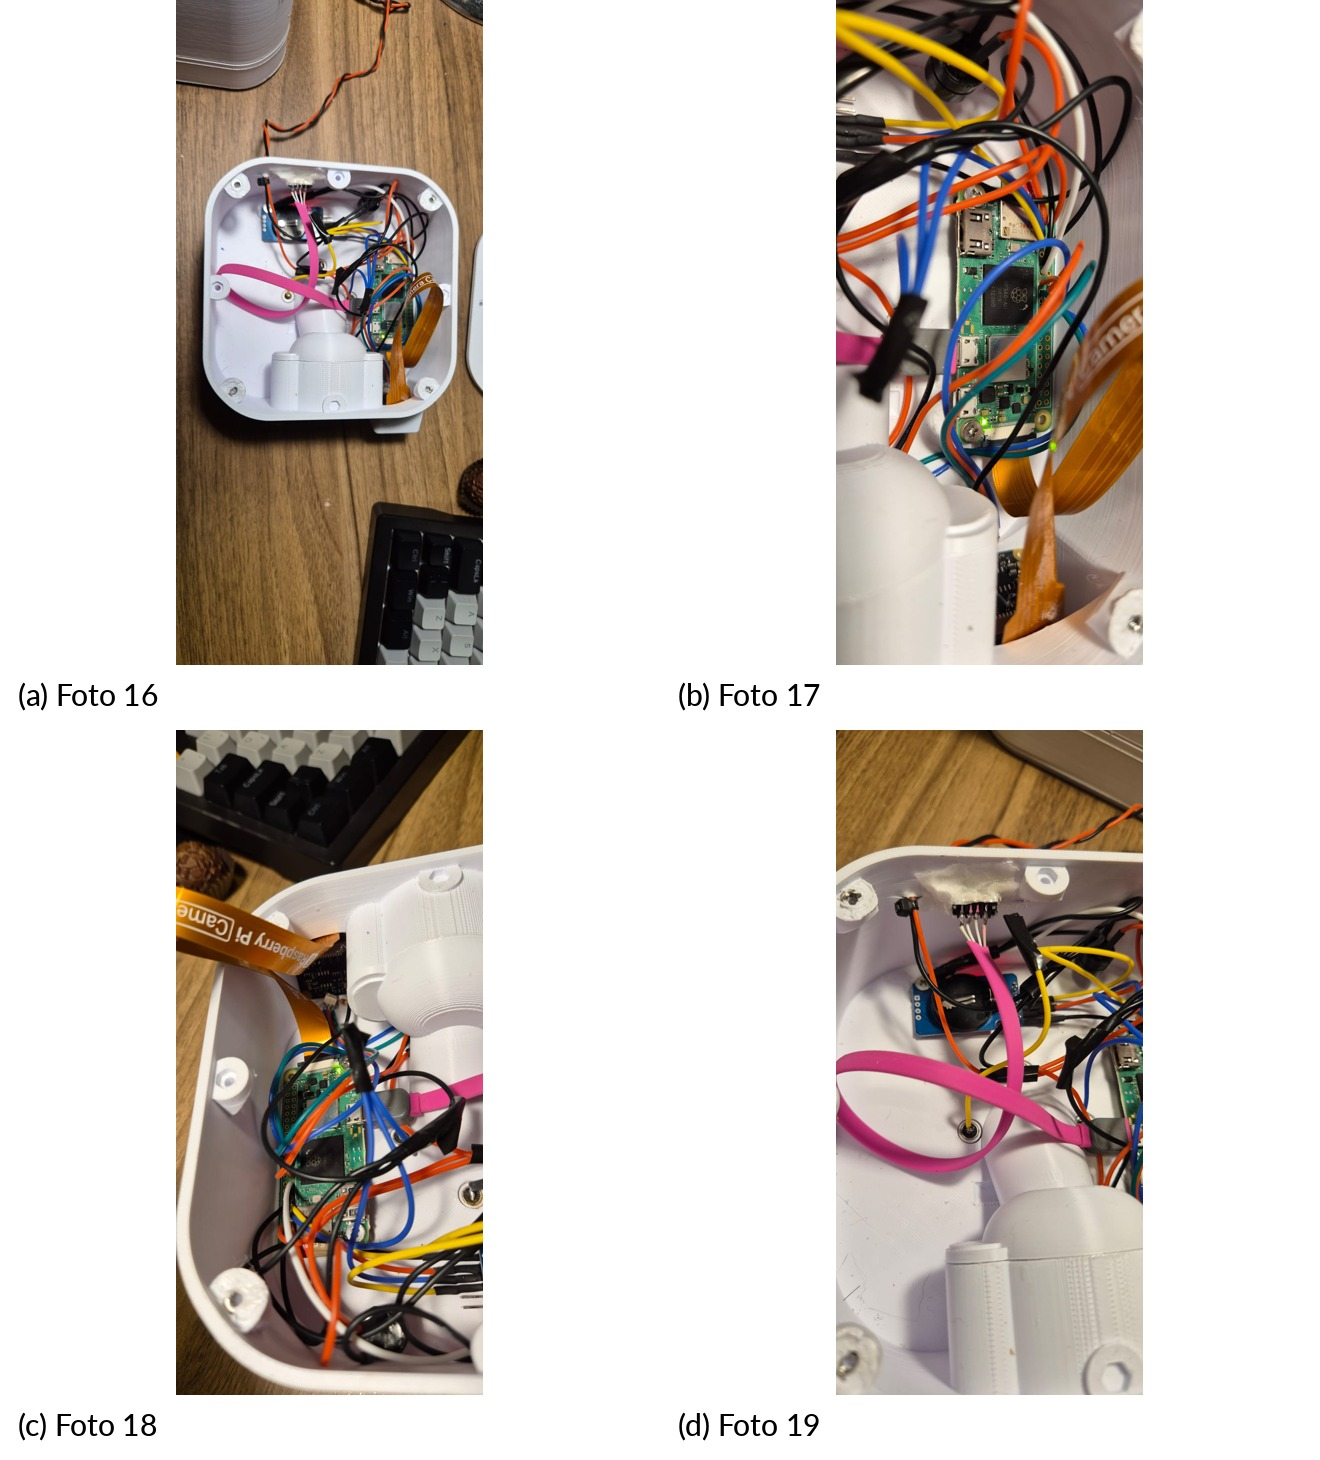
\includegraphics[width=0.98\textwidth,height=0.69\textheight,keepaspectratio]{Figuras/Validacao20261126/central_eletronica.jpg}
\fonte{Acervo dos autores, pacote de validação recebido em novembro de 2026.}
\end{figure}

As Figuras~\ref{fig:int_fisico_2026} e~\ref{fig:int_chicote_2026} permitem relacionar os encaixes, indicadores e chicote à descrição funcional. O I²C comum identifica a placa, não a posição física do encaixe; a associação continua dependente de cadastro e confirmação humana. A orientação dos canais não foi deduzida das cores aparentes nas fotos.

\begin{figure}[htbp]
\centering
\caption{Intermediário: (a) cavidades de encaixe; (b) contatos superiores; (c) LEDs verdes; (d) submódulo encaixado com LEDs azuis}\label{fig:int_fisico_2026}
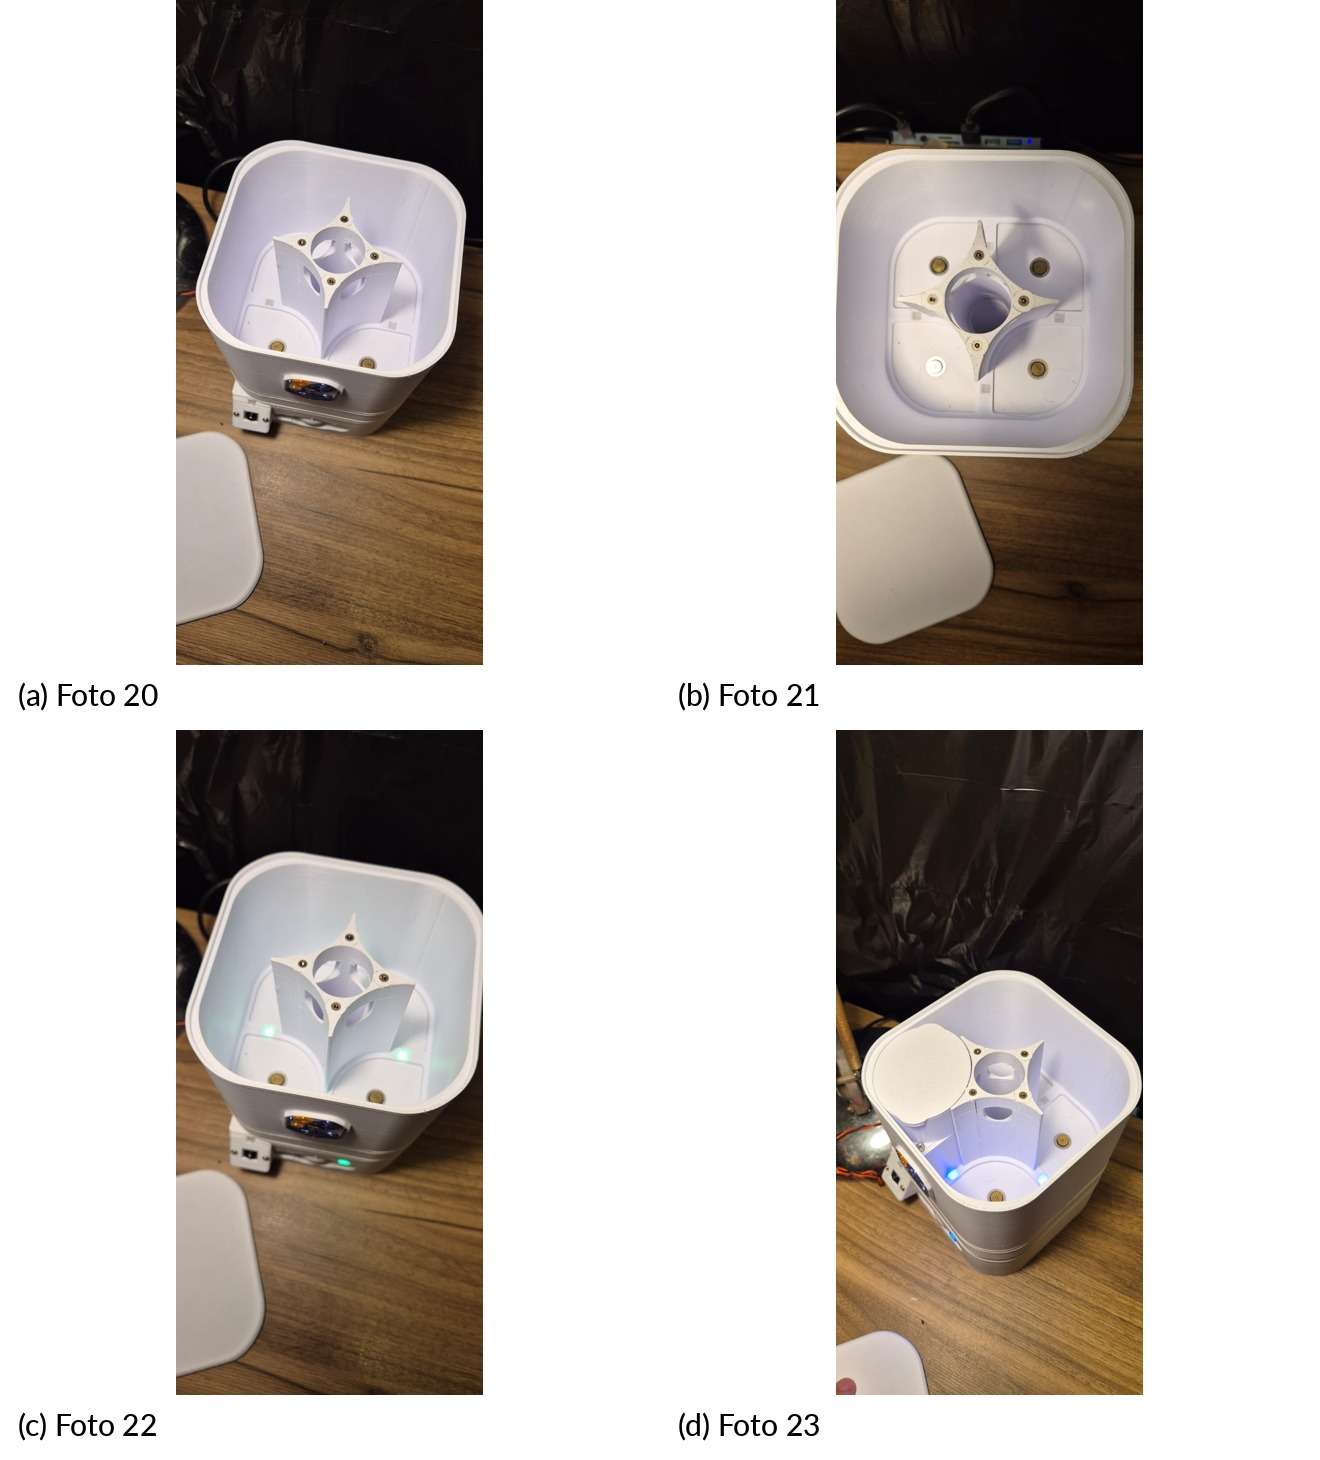
\includegraphics[width=0.98\textwidth,height=0.69\textheight,keepaspectratio]{Figuras/Validacao20261126/intermediario.jpg}
\fonte{Acervo dos autores, pacote de validação recebido em novembro de 2026.}
\end{figure}

\begin{figure}[htbp]
\centering
\caption{Intermediário aberto: (a) submódulo no encaixe; (b) chicote; (c) contatos e ligações inferiores}\label{fig:int_chicote_2026}
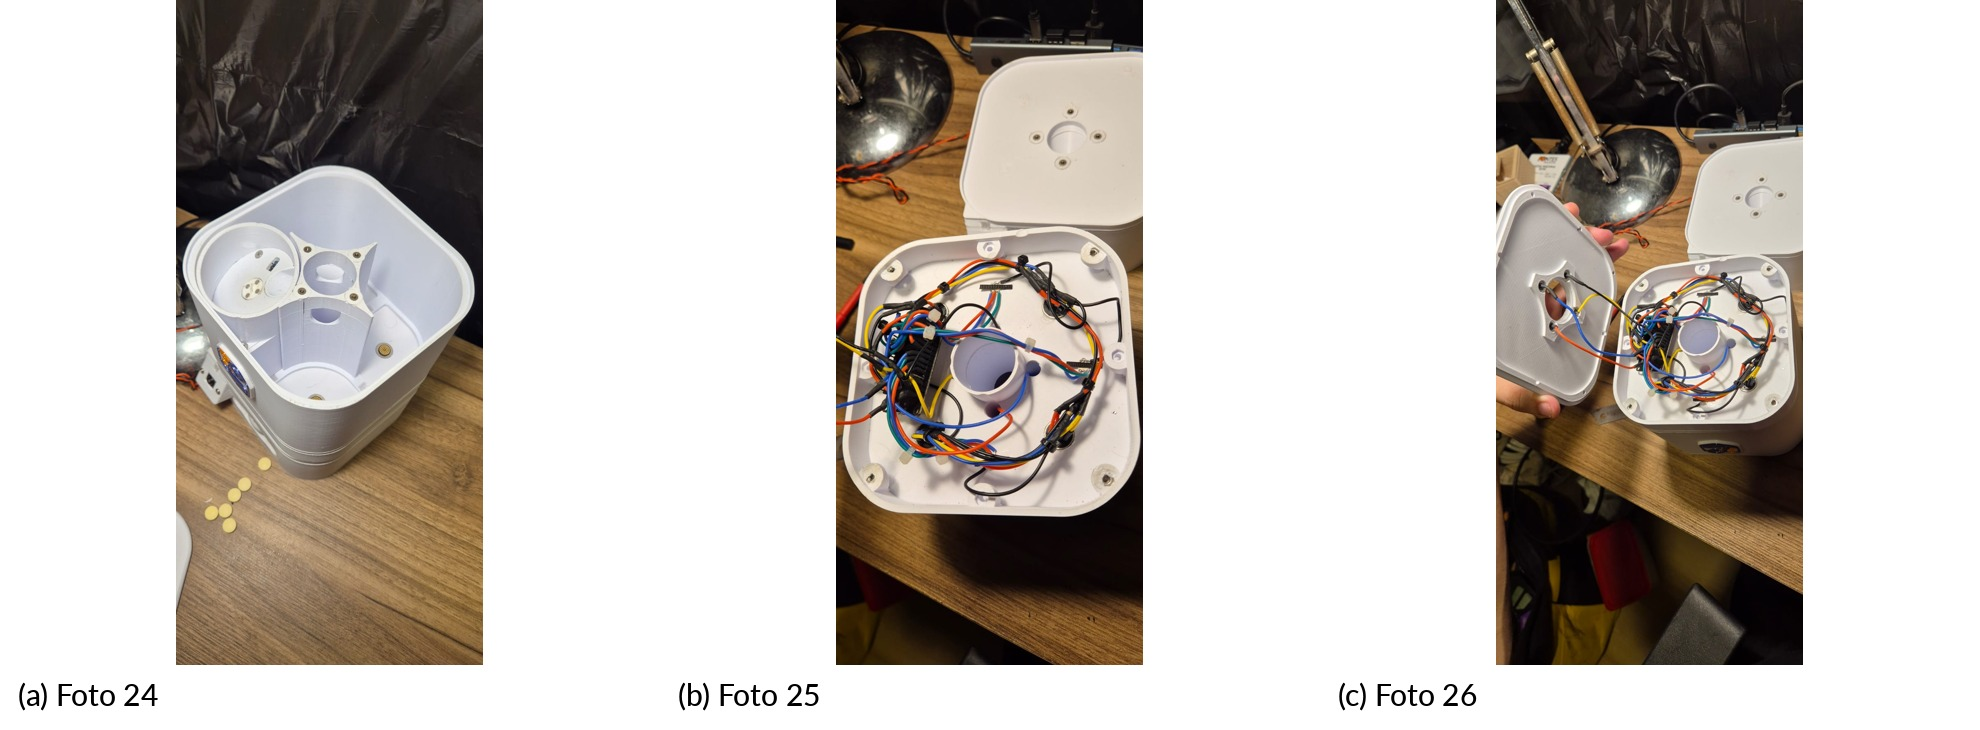
\includegraphics[width=0.98\textwidth,height=0.69\textheight,keepaspectratio]{Figuras/Validacao20261126/intermediario_chicote.jpg}
\fonte{Acervo dos autores, pacote de validação recebido em novembro de 2026.}
\end{figure}

A Figura~\ref{fig:sub_eletronica_2026} documenta ESP32, motor e placa de acionamento do submódulo. Esses registros vinculam a descrição aos componentes montados, sem substituir medições de tensão, corrente ou temperatura sob carga.

\begin{figure}[htbp]
\centering
\caption{Eletrônica do submódulo: (a) motor e driver; (b) ESP32; (c) conjunto 28BYJ-48 e interface de potência}\label{fig:sub_eletronica_2026}
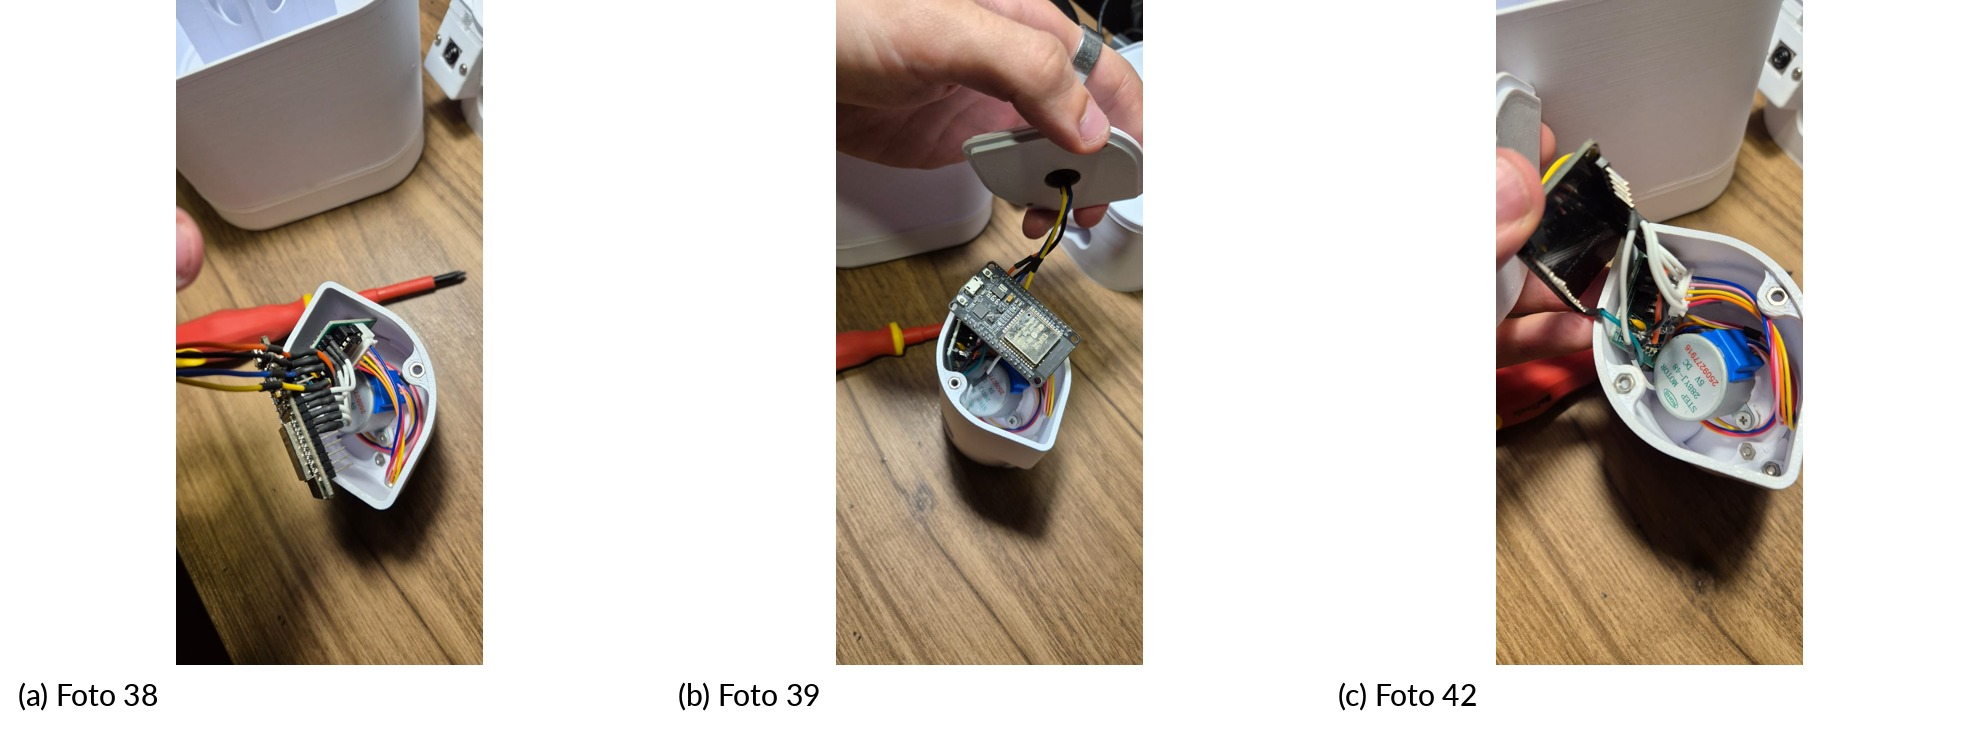
\includegraphics[width=0.98\textwidth,height=0.69\textheight,keepaspectratio]{Figuras/Validacao20261126/sub_eletronica.jpg}
\fonte{Acervo dos autores, pacote de validação recebido em novembro de 2026.}
\end{figure}

\section{Leituras posteriores e limites do diagnóstico elétrico}
Em novembro houve nova perda de comunicação do submódulo durante movimento após os reparos de fiação. O motivo de reinício dessa ocorrência não foi recuperado antes do reencaixe; não se pode atribuí-la conclusivamente ao mesmo brownout do primeiro registro. A recomendação de medir os 5 V junto ao SUB01 durante o giro e avaliar desacoplamento de 470~$\mu$F e 100~nF permanece uma ação de diagnóstico, não uma correção cuja montagem e eficácia estejam demonstradas. \cite{DC_VALIDACAO2026}

Na coleta de 26 de novembro, INT01 e SUB01 voltaram a responder e a telemetria sem motor não mostrou mudança de boot nas amostras válidas. A central ficou entre 53,69~°C e 57,46~°C; as leituras do indicador \texttt{get\_throttled} foram zero. Esses dados descrevem a condição monitorada da Raspberry, não a temperatura de todos os componentes nem a tensão transitória nos contatos. Não substituem ensaio elétrico com carga. \cite{DC_VALIDACAO2026}

\section*{\textcolor{DCPendente}{Complementações necessárias}}
\pendencia{ELE01}{Informar marca/modelo da fonte instalada, etiqueta, regulação, fusíveis, aterramento, proteção e cabeamento. Medir tensão na Pi e nos módulos, queda de tensão, corrente em repouso/atuação e aquecimento. Não tratar 10 A como consumo.}
\pendencia{ELE02}{Conferir ordem, orientação e continuidade real de cada pogo, comprimentos, bitolas e retornos. Completar esquema elétrico pós-reparos e identificar conectores por modelo ou desenho cotado.}
\pendencia{ELE03}{Medir pull-ups equivalentes, capacitância/tempos de subida e níveis do I²C com os módulos e os motores; verificar colisão de endereços, taxas de erro e comportamento no encaixe/retirada energizados. O mapa funcional não atesta integridade elétrica.}
\pendencia{ELE04}{Conferir pinagem do TCRT5000 físico, resistores, alimentação e faixa ADC; obter leituras em cavidade vazia/ocupada e sob diferentes condições. Medir comportamento do motor, driver e sensor em conjunto, sem confundir leitura da cavidade com sensor de saída.}
\pendencia{ELE05}{Confirmar LED adquirido/instalado, terminais A/K, corrente e brilho por cor, resistores e dissipação dos drivers. Fornecer fotos e testes de todas as posições; não assumir funcionamento dos dois intermediários a partir de uma unidade.}
\pendencia{ELE06}{Identificar RTC e bateria realmente instalados; conferir carga e compatibilidade da placa, habilitação no Linux, leitura de /dev/rtc0 e teste após desligamento sem rede. A bateria do RTC não alimenta a Pi.}
\pendencia{ELE07}{Fechar ensaios de buzzer, LEDs centrais, chaveamento, aquecimento, reinício e interferência em conjunto. Inserir esquema final, registros dos instrumentos e condições; confirmar capacitores/proteções acrescentados nos reparos.}
\pendencia{BOM01}{Conciliar os orçamentos XLSX e XLSM/contrato com compras, doações e fretes; o valor anterior de R\$ 2.512,55 não foi localizado e não é adotado. Não preencher custo realizado com orçamento.}
\pendencia{BOM02}{Completar a lista técnica instalada com sensores, conectores pogo, resistores, drivers de LEDs, buzzer/MOSFET, RTC, bateria, cabos, proteções e demais itens. Conferir a troca de WS2812B cotado pelo RGB comum documentado.}

% Revisão consolidada: 25/11/2026. Não antecipa resultados finais.
\chapter{Programação embarcada}
\section{Organização do firmware e papéis}
A documentação separa dois perfis: intermediário e submódulo. O primeiro administra sinalização e posição; o segundo controla motor e sensor. Bibliotecas e constantes compartilhadas descrevem o protocolo, estados e validações. O mesmo número de GPIO pode ter função diferente entre os papéis, motivo pelo qual configuração e firmware precisam estar associados à placa correta. \cite{DC_COMPILADO,DC_CIRCUITOS}
\section{Inicialização e configuração persistente}
O firmware documentado utiliza configuração persistente com papel, instância, endereço e identificador do local de operação, além de mecanismos de integridade e leitura de retorno. O registro de inicialização distingue um novo boot de uma resposta antiga. Parâmetros gravados e lidos na placa são a evidência pertinente; um arquivo-fonte isolado não comprova o que está instalado. \cite{DC_COMPILADO}
\section{Comunicação e estado}
O protocolo DC1 utiliza quadros de 32 bytes, marcadores, versão, identificadores, campos reservados e CRC-8 de polinômio 0x07. A validação deve preceder o efeito físico. CRC correto não equivale a autorização criptográfica e não substitui as condições de segurança locais. O ACK de aplicação no protocolo também deve ser distinguido do reconhecimento elétrico do I²C. \cite{DC_COMPILADO}
\section{Controle do motor e tratamento de duplicatas}
Os GPIO27/26/25/33 comandam o driver segundo a sequência configurada; a conversão entre fases e deslocamento precisa ser calibrada na montagem. A documentação exige limite local de fases e duração, manutenção de resultado pendente e recuperação após perda de resposta. Um resultado desconhecido exige reconciliação, não o reenvio cego de um novo movimento. \cite{DC_COMPILADO}
\section{Leitura e calibração óptica}
O GPIO32/ADC1 recebe a leitura reflexiva. A avaliação exige referência de cavidade vazia/ocupada, associação com fase, condições de iluminação e verificação independente. O material relata evolução para localização e verificação de cavidades, mas isso não permite presumir calibração válida após troca de disco, reinício ou intervenção mecânica. \cite{DC_COMPILADO}
\section{Atualização das ESP32}
O acervo descreve atualização pelo barramento, com transmissão segmentada, conferência de integridade, ativação e recuperação. Há diferença entre testes do atualizador, transmissão à placa, reinício e confirmação da nova versão. Atualização bem-sucedida de uma placa não demonstra aceitação de todas as unidades. \cite{DC_COMPILADO}
\section{Versões e evidências necessárias}
No registro de 12/11 constam INT-01 0.3.1 e SUB-01 0.6.1. Esse registro é posterior aos firmwares iniciais e deve ser conservado como evidência datada, sem declarar que continua sendo a configuração atual. \cite{DC_ANALISE}
\pendencia{EMB01}{Fornecer código/release final, hashes, dependências e manifesto de gravação por placa; papel, instância, endereço, site, boot ID e versão lida após reinício.}
\pendencia{EMB02}{Completar tabela de estados, operações, códigos de erro e limites efetivamente ativos na versão final. Relacionar cada estado às saídas seguras e condições de recuperação.}
\pendencia{EMB03}{Anexar parâmetros e registros de calibração e localização do disco utilizado: fases por volta, intervalo, leituras, limiares, dispersão, falhas e restauração após desligamento.}
\pendencia{EMB04}{Fornecer relatórios de bancada de motor/sensor, duplicatas, perda de comunicação, reinício durante movimento, falha de persistência e recuperação. Separar teste simulado de execução física e identificar denominadores.}
\pendencia{EMB05}{Comprovar atualização pelo barramento e recuperação de interrupção/corrupção com logs sanitizados. Não assumir assinatura, rollback ou persistência preservada sem evidência da versão.}

% Revisão consolidada: 25/11/2026. Não antecipa resultados finais.
\chapter{Servidor e execução local}
\section{Responsabilidades e persistência}
A Raspberry Pi mantém a coordenação local entre agenda, firmware, periféricos e servidor. A documentação descreve persistência em SQLite, filas de eventos e sincronização pela API. Essa organização busca tolerar indisponibilidade de rede, mas a ativação da agenda depende de identidade, associação física, tempo confiável e comissionamento. \cite{DC_COMPILADO}
\section{Agenda, comandos e reconciliação}
Um comando digital deve ser vinculado à intenção, às pré-condições, à execução e ao resultado. Receber um comando não demonstra dispensação; finalizar um giro não demonstra saída; observação visual não demonstra ingestão sem critério definido. A documentação separa estados e impede repetição automática quando o resultado do mecanismo permanece incerto. \cite{DC_COMPILADO}
\section{Rede e provisionamento}
O projeto prevê configuração da rede por Bluetooth pelo celular e recuperação quando não há Wi-Fi utilizável, além de fluxos de reinício e recadastramento sem botão físico. As credenciais e a identidade do dispositivo devem ser protegidas e preservadas conforme o tipo de operação. O ensaio precisa identificar o telefone, navegador, versão, rede e respostas observadas. \cite{DC_COMPILADO}
\section{Sinalização e modo de demonstração}
Os LEDs e o buzzer são saídas locais; suas convenções precisam corresponder às mensagens no aplicativo. O registro de novembro descreve também modo palco, com cenas de luz e som sem motor. Esse modo deve ser identificado como demonstração de sinalização, não como ensaio de dispensação ou de agenda automática. \cite{DC_ANALISE}
\section{Atualização e rastreabilidade}
A execução local evoluiu por pacotes e instalações registradas. O relatório de novembro identifica runtime 0.7.12 na Pi, enquanto o checkout do servidor ainda indicava 0.7.7. Isso evidencia a necessidade de registrar a origem e o hash da versão instalada, sem usar o número do checkout como substituto automático do estado da Pi. \cite{DC_ANALISE}
\section{Limitações de operação local}
O mesmo relatório informa relógio confiável por NTP, sem RTC, \texttt{hardware\_ready=false} e bloqueios de agenda ligados a comissionamento, localização e perfil. Portanto, a monografia não afirma funcionamento automático offline aceito. O objetivo RNF01 continua formalmente exigido, mas seu atendimento precisa de teste específico. \cite{DC_ANALISE}
\pendencia{BE01-RUNTIME}{Confirmar release e hash instalados na data de fechamento, manifesto, dependências, serviços e configuração efetiva. Documentar o provisionamento ativo e a diferença entre fonte no servidor e instalação local.}
\pendencia{BE02-AGENDA}{Fornecer evidência de comissionamento, tempo confiável sem rede, calibração, associação e pré-condições da agenda. Manter a declaração de operação automática pendente até ensaio de perda de rede, reinício e recuperação.}
\pendencia{BE03-REDE}{Anexar roteiros e logs de pareamento, configuração/troca de Wi-Fi, senha incorreta, perda de conexão, reset e recadastramento, sem expor segredos.}
\pendencia{BE04-LOCAL}{Comprovar persistência de filas e idempotência, tratamento de resultado incerto, sincronização após falha e atualização segura da Pi com interrupção controlada.}

\section{Serviços e fluxo de cuidado}
A API FastAPI concentra regras e intermedia os dados usados pelo Care e pela Raspberry Pi. O acervo descreve PostgreSQL/Supabase para os dados centrais e autenticação, enquanto o dispositivo mantém sua persistência local. A arquitetura isola a atuação do motor da interface web e de respostas do agente. \cite{DC_COMPILADO,DC_APP}
\section{Modelo lógico e eventos}
Os documentos descrevem pacientes, medicamentos, estoque, rotinas, atividades, observações, dispositivos, comandos e eventos. Esses conceitos não são equivalentes: uma rotina é um plano; uma observação pode ser um relato; e um evento deve indicar origem e instante. Campos de dosagem textual e quantidade física por tomada também têm significados distintos. \cite{DC_COMPILADO,DC_FOUNDRY}
\section{Autenticação e autorização}
O login do aplicativo é obrigatório, conforme confirmação da autora. Os materiais descrevem JWT e autenticação do dispositivo, mas a documentação também registra uma conta de cuidado compartilhada em determinada versão. Não se presume segregação multiusuário ou autorização por paciente apenas pela existência de telas denominadas cuidador e paciente. \cite{DC_APP,DC_COMPILADO}
\section{Idempotência e sincronização}
O servidor recebe comandos e eventos e deve preservar identificadores e resultados. Em falhas ambíguas, a aplicação precisa consultar o estado antes de reenviar uma intenção que possa produzir efeito físico ou nova gravação. Hashes e normalização dos dados devem ser equivalentes entre os participantes e vinculados à versão do contrato. \cite{DC_COMPILADO}
\section{Implantação, manutenção e limites}
O relatório de 12/11 descreve serviços ativos, porém registra ocupação de disco de 98\%, crescimento associado à telemetria, ausência de purga confirmada e checkout com alterações não versionadas. Esses números são históricos e não constituem medição desta revisão. A disponibilidade naquele instante não demonstra disponibilidade contínua nem recuperação de desastre. \cite{DC_ANALISE}
\pendencia{BE01-API}{Fornecer versão e hash da API, migrações aplicadas, esquema do banco, configuração sanitizada e manifesto dos serviços na versão final. Não atribuir versão do runtime à API.}
\pendencia{BE02-CONTRATO}{Conferir os contratos atuais API--Pi, normalização de payload/hash, estados, paginação e migrações. O compilado indica uso de cancelled em fluxos de demonstração; confirmar que o tipo/coluna de produção o aceita e registrar a migração.}
\pendencia{BE03-SEGURANCA}{Documentar autorização real por usuário/paciente, expiração/renovação de sessão, rotação de segredos, retenção e purga. Fornecer teste de backup/restauração e política para imagens/eventos.}
\pendencia{BE04-TESTES}{Anexar resultados próprios do servidor, migrações e integração autenticada: data, ambiente, versões, comandos, aprovados, falhas e limites de simulação. Não converter relatórios históricos em aceite final.}


% Interface Care: capítulo próprio, sem duplicação do servidor.
\chapter{Aplicativo Care}

\section{Papel, tecnologias e tarefas}
O Care é a interface web de configuração e acompanhamento do DoseCerta. A documentação identifica React e TypeScript, com acesso às operações de cuidado por meio da FastAPI. Os materiais descrevem pacientes, dispositivos, medicamentos, estoque, agendas, atividades, observações e histórico; cada tarefa deve ser confirmada na versão entregue. Telas ilustrativas não demonstram sucesso de integração autenticada ou execução no hardware. \cite{DC_APP}
\section{Login e fluxo de informação}
O login é obrigatório, conforme confirmação da autora. A documentação associa Supabase à autenticação e descreve JWT; as operações de cuidado passam pela API. A monografia não presume acesso direto da interface às tabelas de cuidado, autorização individual por paciente ou proteção multiusuário não demonstrada. \cite{DC_APP,DC_COMPILADO}
\section{Estados e tratamento de falhas}
A interface deve diferenciar plano, comando enviado, confirmação do dispositivo, observação e resultado inconclusivo. Repetir uma ação após falha de rede pode produzir efeito duplicado, motivo pelo qual confirmação e reconciliação precisam corresponder ao contrato do servidor. O modo palco e a simulação devem ser identificados como tais, sem se confundirem com dispensação física. \cite{DC_APP,DC_ANALISE}
\section{Evidências e avaliação da interface}
A documentação do aplicativo esclarece que as contagens históricas de outras suítes não incluem resultados próprios do Care. É necessário testar interface, API autenticada, dispositivo e acessibilidade de forma separada e depois integrar os fluxos. Avaliação de uso com pessoas exige protocolo e autorizações aplicáveis. \cite{DC_APP}
\pendencia{APP01}{Nicolas: a autora enviará a versão e as telas do aplicativo. Inserir release/hash, ambiente, navegação e tarefas efetivamente disponíveis, além de capturas sanitizadas.}
\pendencia{APP02}{Login obrigatório confirmado: inserir telas e evidências do fluxo real, emissão/validação e renovação de sessão, expiração, logout, acesso negado e mensagens de erro, sem expor credenciais.}
\pendencia{APP03}{Conferir a autorização na versão final, especialmente se as visões de paciente/cuidador usam conta única. Não declarar isolamento de dados sem teste.}
\pendencia{APP04}{Fornecer resultados próprios da suíte Care, integração autenticada, estados de erro/sem rede, atualização de histórico e comunicação com o aparelho. Identificar o que foi simulado.}
\pendencia{APP05}{Inserir fotos/capturas atualizadas das tarefas principais e avaliação de acessibilidade/usabilidade: método, participantes quando houver, critérios, problemas e correções. Não inferir qualidade de uso pelo desenho das telas.}

\chapter{Visão computacional}\label{cap:visao}
A visão computacional compõe a observação associada à tomada, em complemento aos registros do mecanismo e aos relatos do cuidado. Sua função é produzir uma saída rastreável sobre as imagens analisadas, preservando a condição inconclusiva quando não houver informação suficiente. Uma observação visual não é tratada como comprovação clínica de ingestão.

A integração com a central compartilha o recurso de câmera e precisa delimitar aquisição, processamento e devolução do resultado. O registro deve conservar o evento de referência, a versão do método e as condições da captura, de forma que a saída possa ser relacionada à rotina apresentada no aplicativo.

\section{Método de aquisição e processamento}
\pendencia{VIS01}{Completar a descrição técnica da frente de visão com o objetivo operacional e o evento observado. Responsável: Vinicius.}
\pendencia{VIS02}{Inserir a arquitetura implementada: aquisição, preparação, algoritmo ou modelo, saídas, erros, versões e implantação. Acrescentar o diagrama e as imagens do método utilizado.}
\section{Dados e avaliação}
\pendencia{VIS03}{Informar origem e autorização dos dados, anonimização, classes, rotulagem, composição e separação dos conjuntos e referência independente.}
\pendencia{VIS04}{Definir métricas, limiares, cenários, repetições, condições e critérios de aceitação. Distinguir a pontuação do modelo de certeza clínica.}
\section{Resultados e limitações}
\pendencia{VIS05}{Inserir somente os resultados experimentais efetivamente obtidos, com versões, denominadores e registros correspondentes.}
\pendencia{VIS06}{Descrever as falhas observadas, fatores de generalização e condições em que o método deve declarar resultado inconclusivo.}

\chapter{Agente de inteligência artificial}\label{cap:agente}
O agente oferece uma forma de consultar informações e solicitar ações do cuidado em linguagem natural. Sua função é complementar o aplicativo, não prescrever, escolher doses ou substituir o responsável pelo tratamento. A execução das solicitações permanece sujeita às regras da API e às permissões do contexto.

\section{Evolução e organização}
A proposta inicial utilizou Microsoft Copilot Studio. O desenvolvimento posterior passou a utilizar Microsoft Foundry, com um agente de conversa e uma configuração separada de teste para ferramentas MCP. Essa evolução alterou o modo de integrar voz, contexto e operações de escrita. \cite{DC_ARTIGO,DC_FOUNDRY}

Na configuração de referência de 3 de novembro de 2026, o aplicativo utilizava o agente de conversa na versão 5, sem MCP. A configuração de teste utilizava \texttt{tcc-agent-mcp-teste} na versão 8. A Figura~\ref{fig:agente_arquitetura} apresenta os dois caminhos. A separação evita atribuir à interface de voz funções disponíveis apenas no ambiente de teste.

\begin{figure}[htbp]
\centering
\caption{Separação entre o assistente do aplicativo e o agente de teste com MCP}\label{fig:agente_arquitetura}
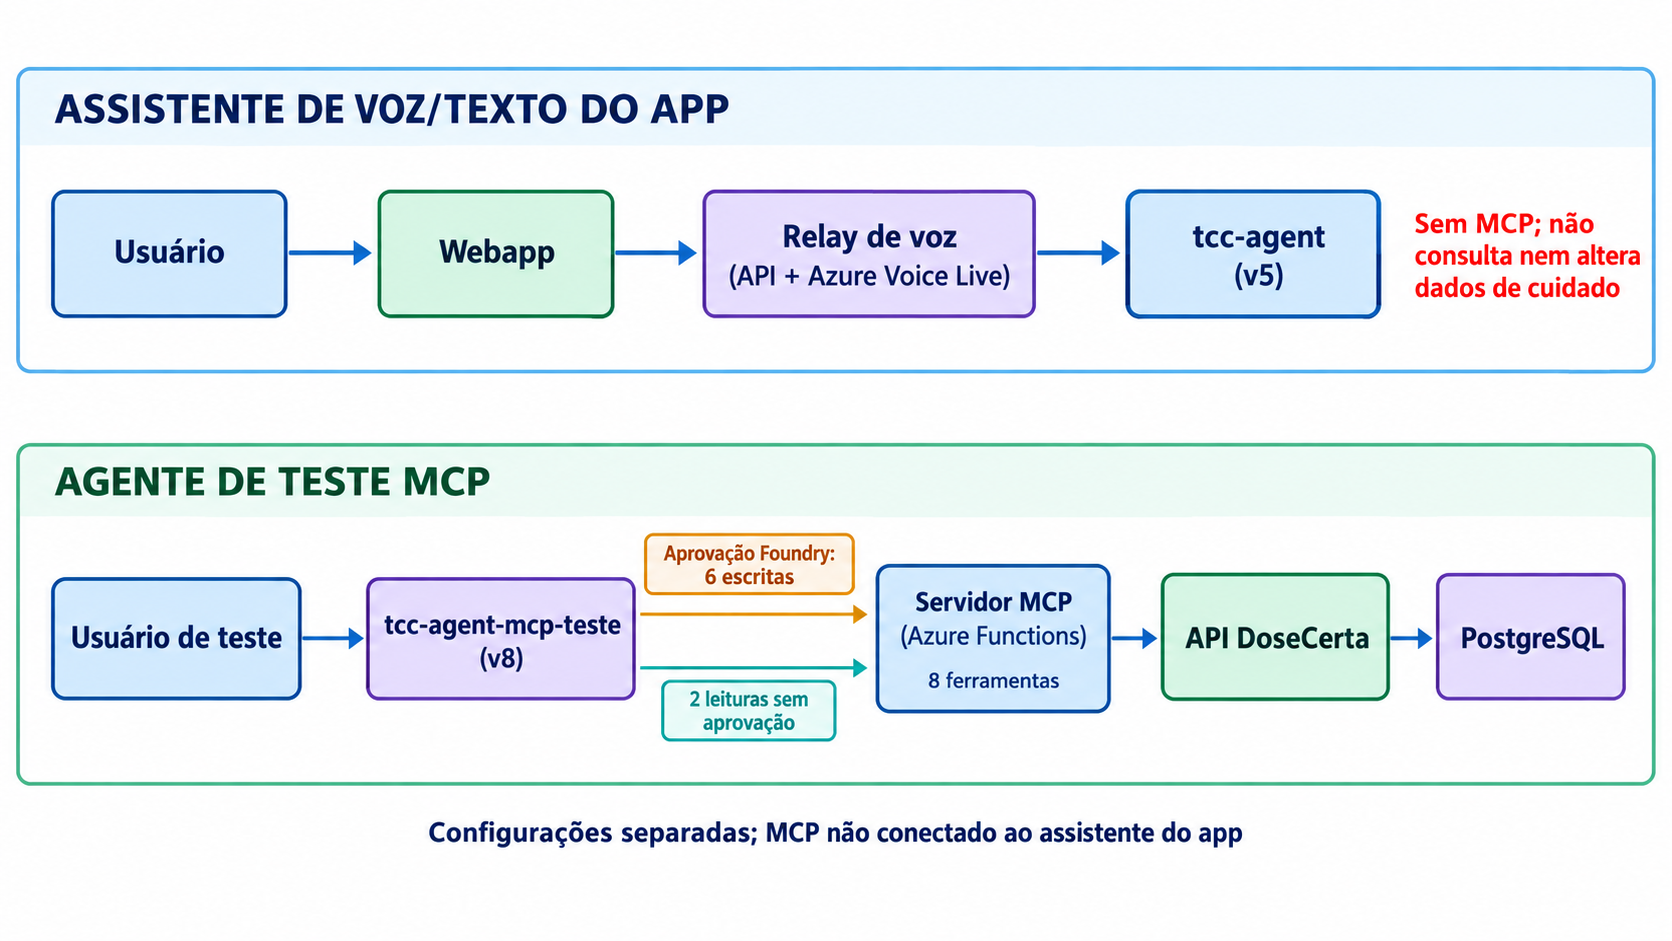
\includegraphics[width=0.98\textwidth,height=0.66\textheight,keepaspectratio]{Figuras/SharePoint/agente_arquitetura.png}
\fonte{Elaboração dos autores. Configuração de referência de 3 nov. 2026.}
\end{figure}


\section{Contexto e recuperação de informações}
Na configuração de referência de 3 de novembro, o agente de conversa utilizava pesquisa em arquivos para recuperar contexto. A utilidade desse recurso depende da seleção, da revisão e da atualização do conteúdo disponibilizado. A existência de um índice não garante que o manual esteja completo ou que os registros atuais do cuidado sejam consultados.

As respostas devem distinguir conhecimento de referência e dados obtidos por ferramenta. Quando uma consulta falha ou retorna informação parcial, o agente precisa informar esse limite antes de afirmar rotina, estoque ou histórico. Textos recuperados são tratados como dados de contexto, não como instruções para alterar a política de operação.

\section{Ferramentas e operações}
A configuração MCP de referência de 3 de novembro reunia duas ferramentas de leitura e seis de escrita. As leituras consultam contexto e registros; as escritas alteram cadastros, rotinas, atividades ou observações. A Tabela~\ref{tab:13-1} apresenta os identificadores da configuração de referência. \cite{DC_FOUNDRY}

{\small\setlength{\tabcolsep}{3pt}\begin{longtable}{p{0.44\textwidth}p{0.12\textwidth}p{0.32\textwidth}}\caption{Ferramentas da cópia MCP do agente, documentadas em novembro}\label{tab:13-1}\\
\hline
\textbf{Ferramenta documental} & \textbf{Tipo} & \textbf{Papel}\\\hline
\endfirsthead\hline
\textbf{Ferramenta documental} & \textbf{Tipo} & \textbf{Papel}\\\hline
\endhead
\texttt{get\_care\_context} & Leitura & Contexto de cuidado\\\hline
\texttt{list\_care\_records} & Leitura & Registros de cuidado e histórico\\\hline
\texttt{create\_medication\_schedule} & Escrita & Criação de rotina\\\hline
\texttt{update\_medication\_schedule} & Escrita & Alteração de rotina\\\hline
\texttt{update\_medication} & Escrita & Alteração de medicamento\\\hline
\texttt{add\_care\_observation} & Escrita & Registro de observação\\\hline
\texttt{create\_daily\_activity} & Escrita & Criação de atividade\\\hline
\texttt{update\_daily\_activity} & Escrita & Alteração de atividade\\\hline
\end{longtable}}{\small\noindent Fonte: Configuração do agente em 3 nov. 2026.\par}

As operações de escrita requerem esclarecimento dos dados necessários e aprovação antes da execução. Uma frase ambígua sobre dosagem ou horário não deve ser convertida diretamente em alteração. A confirmação apresenta a ação e seus argumentos, permitindo ao usuário revisar o pedido.

\section{Aprovação e segurança}
O fluxo da Figura~\ref{fig:agente_aprovacao} começa pela consulta do contexto e pela verificação da clareza do pedido. A negação da aprovação encerra a ação sem escrita. A aprovação, por sua vez, permite prosseguir para o servidor, mas não elimina a validação das regras de negócio e das permissões.

\begin{figure}[htbp]
\centering
\caption{Solicitação, esclarecimento, aprovação e execução de uma operação de escrita}\label{fig:agente_aprovacao}
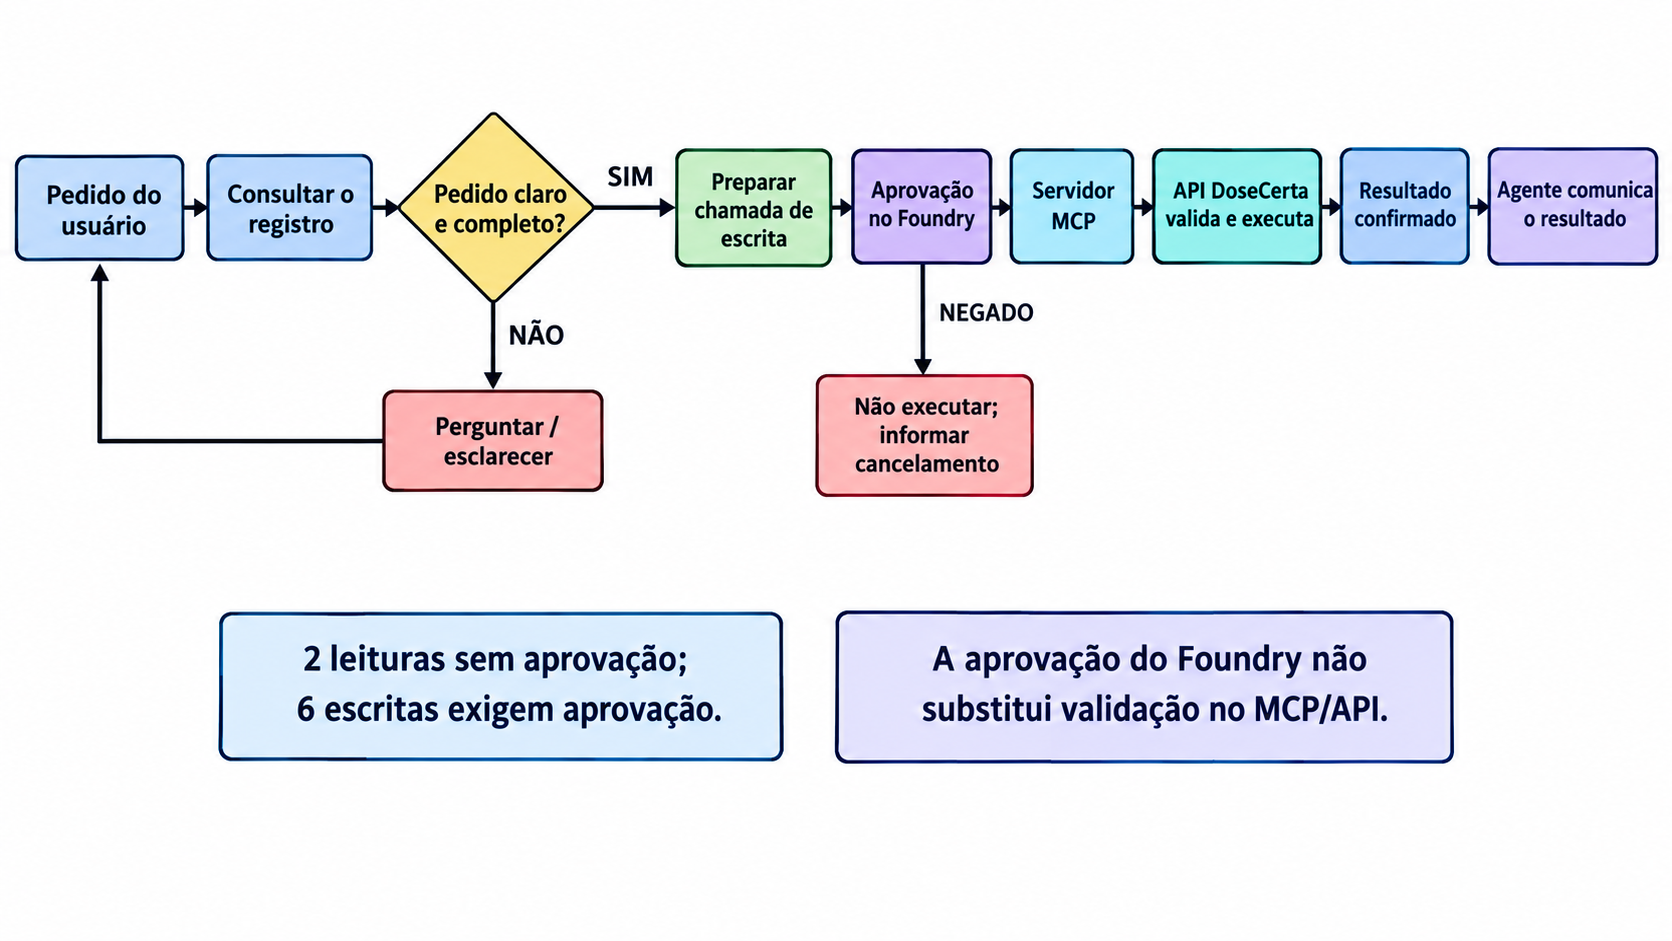
\includegraphics[width=0.98\textwidth,height=0.66\textheight,keepaspectratio]{Figuras/SharePoint/agente_aprovacao.png}
\fonte{Elaboração dos autores (2026).}
\end{figure}


A segurança é distribuída entre identificação do usuário, autorização do serviço e validação na API. Instruções no prompt complementam esses controles, mas não os substituem. Chaves e credenciais não integram o texto nem as capturas públicas.

Quando o retorno de uma ferramenta é incerto, o agente deve consultar o estado antes de solicitar repetição. O mesmo cuidado se aplica à comunicação do resultado: preparar uma chamada, obter aprovação, persistir a alteração e produzir eventual efeito físico são etapas diferentes.

\section{Voz e integração com o Care}
A interface de voz utiliza um relay no backend. Na configuração histórica de 3 de novembro, esse caminho não processa as aprovações exigidas pelas ferramentas MCP, motivo pelo qual foi mantido separado do agente de teste. A resposta conversacional disponível no Care não é, portanto, apresentada como execução automática das oito ferramentas. \cite{DC_FOUNDRY,DC_ANALISE}

A integração deve conservar os caminhos manuais do aplicativo e informar o que foi efetivamente realizado. O agente pode esclarecer uma solicitação, consultar e apresentar um retorno, mas não deve transformar uma falha de acesso em afirmação de ausência de dados.

\section{Avaliação}
A avaliação diferencia recuperação de contexto, escolha da ferramenta, argumentos, confirmação, autorização e efeito persistido. Também considera respostas a ambiguidades, recusa de pedidos clínicos e tratamento de falhas. O teste funcional do servidor MCP avalia uma parte dessa cadeia; não representa, isoladamente, a qualidade do modelo ou da experiência de voz.

Os procedimentos são relacionados à estratégia de integração do capítulo seguinte. Os resultados do agente devem manter a versão, o ambiente e os casos utilizados, permitindo interpretar o alcance de cada evidência.

\section{Estado da integração e alcance da evidência}
Os novos insumos não apresentam uma campanha de interações do modelo que permita estimar precisão de seleção de ferramenta, frequência de falso sucesso ou segurança de escritas em contexto real. A suíte do MCP verifica componentes de software, não corresponde ao mesmo número de conversas avaliadas. A conversa de leitura documentada e a configuração de aprovação são evidências distintas de uma alteração aprovada, persistida e conferida no cuidado correto. \cite{DC_VALIDACAO2026}

A aprovação do Foundry é uma política do caminho do agente, não uma trava universal de toda chamada ao MCP. Quem detiver a chave do serviço pode estar fora desse caminho; por isso, controle de segredo, autorização na API e registro da origem permanecem necessários. A monografia não presume que a integração entre voz, MCP e Care esteja validada apenas porque cada parte responde isoladamente. \cite{DC_VALIDACAO2026}

\section{Relatos posteriores à configuração de referência}
O pacote de novembro relata migração do agente para Azure Voice Live, desligamento do MCP dedicado anterior e consulta somente de leitura ao contexto do paciente por \texttt{GET /v1/care/assistant\_context}; as alterações permaneceriam no aplicativo. Essas informações são relatos de integração de outra frente, não uma atualização confirmada da configuração do agente neste capítulo. Não se apresentam a leitura de receita nem a redução de latência de 94,5 s para 11,0 s como métricas verificadas sem versão, cenário, repetição e registro primário. \cite{DC_VALIDACAO2026}

\section*{\textcolor{DCPendente}{Complementações necessárias}}
\pendencia{AG01}{Confirmar modelo, parâmetros e versões finais do agente publicado e do agente chamado pelo aplicativo. O rótulo interno gpt-5.6-luna precisa de identificação verificável e não deve ser tratado como especificação pública do modelo.}
\pendencia{AG02}{Fornecer evidências das oito ferramentas, aprovação e recusa de escritas, validação do servidor, tratamento de duplicatas e falhas ambíguas. Não executar gravações de teste em dados reais.}
\pendencia{AG03}{Inventariar o conteúdo efetivo do armazenamento vetorial: fontes, revisão, atualização e avaliação da recuperação, incluindo manual atual. Não assumir base atualizada por existir \texttt{file\_search}.}
\pendencia{AG04}{Anexar diálogos sanitizados e registros de chamadas/efeitos persistidos em ambiente de teste; identificar resultado parcial, erro, restauração e limpeza dos dados de teste.}
\pendencia{AG05}{Definir e executar conjunto de avaliação do agente: casos, repetições, referência humana, critérios, falhas clínicas e resultados. Contagens de testes do MCP não são desempenho do modelo.}
\pendencia{AG06}{Documentar permissões, rotação de chaves, limites de acesso, retenção e proteção contra instruções maliciosas em dados. Distinguir controles verificáveis de orientações do prompt.}
\pendencia{AG07}{Reconciliar a configuração histórica de 03/11 com o relato posterior de Voice Live e ferramenta de contexto somente de leitura; identificar versão ativa, protocolo, permissões e evidência no Care antes de afirmar a integração atual.}

\section{Método de integração e testes}\label{cap:testes}
A avaliação foi organizada em inspeção de projeto, testes automatizados, execução nas placas e integração de ponta a ponta. O desenvolvimento incluiu testes de caixa preta, exercitando entradas, saídas e estados observáveis, e de caixa branca, verificando regras internas, persistência e tratamento de erros. O procedimento distingue testes executados durante o desenvolvimento do protocolo controlado ainda a concluir.

\subsection{Preparação, configuração e unidade de ensaio}
Antes de cada bloco, devem ser registrados revisão mecânica, disco, unidade física de teste, alimentação, versões de firmware/runtime/API/Care, ambiente e política de travas. A referência temporal, a calibração, a identidade dos módulos e a ausência de operação incerta são condições de preparação. Instrumento, operador e responsável pela observação acompanham o registro.

Uma tentativa de dispensação corresponde a um pedido identificado e seu desfecho, inclusive quando recusado ou interrompido. ``Unidade de teste'' designa o objeto físico usado no ensaio, com tipo e dimensões identificados; não significa necessariamente medicamento destinado a ingestão. O número de pedidos, de ciclos internos, de unidades solicitadas e de unidades coletadas é conservado separadamente.

\subsection{Dispensação com contagem independente}
A campanha controlada consiste em repetir um roteiro sob condições registradas, mantendo constantes as características escolhidas para o bloco. A quantidade no copo é contada por observação física, sem adotar como verdade o estado do motor, a leitura do sensor ou a baixa no aplicativo. Essa é a referência independente. Sua comparação com o pedido permite identificar acerto, ausência, unidade extra, retenção, travamento e resultado não observado.

O procedimento compreende conferir o estoque inicial, identificar o pedido, executar sem reenvio indevido, contar o coletor, registrar tempo e condição do mecanismo e conferir os estoques físico e digital. Fotografias identificadas apoiam a auditoria. Ausência de observação não é registrada como zero. Mudança de peça, ajuste ou versão inicia novo bloco; não elimina falhas do anterior. Fichas e proposta de blocos estão no Apêndice~\ref{ap:ensaios}.

\subsection{Mecânica, elétrica e sensoriamento}
A inspeção dimensional compara as cotas nominais V75 às medidas da peça impressa, sem inferir tolerância apenas da malha. A avaliação elétrica considera polaridade, continuidade, tensão e corrente em repouso e atuação, quedas nos contatos e aquecimento. Remoção energizada exige ensaio próprio; reconexão lógica não comprova segurança elétrica.

Para o sensor, a referência é a inspeção da cavidade vazia e ocupada, com o reservatório montado. Localização, calibração e restauração de posição são avaliadas em condições identificadas, inclusive perda de referência. Resultados de ADC parado não são extrapolados para o mecanismo em movimento.

\subsection{Software, comunicação e atualização}
As suítes automatizadas verificam estados, contratos, identidade, quadros válidos e inválidos, CRC, duplicatas e persistência. No aplicativo, consideram componentes, navegação e API simulada; no servidor, regras, contratos e gravação. Os registros conservam comando de execução, versão, casos aprovados, falhas, erros e ignorados. Rodadas sobrepostas não são somadas.

Em placa, são considerados parada, perda de resposta, reinício durante movimento, resultado retido e reconciliação. Atualizações são avaliadas por transferência, verificação de integridade, ativação, reinício e recuperação. Para a Pi, verifica-se também assinatura; nas ESP32, SHA-256 não é apresentado como assinatura. Os testes com dependências simuladas são distinguidos da atuação física.

\subsection{Integração Care--API--central e recuperação}
O roteiro acompanha uma sessão autenticada desde a solicitação até comando, atuação, confirmação humana, estoque e histórico, utilizando a mesma identidade de operação. Perda de rede, resposta tardia, expiração de sessão, duplicata e reinício são tratados junto à recuperação. Na operação sem internet, é preciso verificar relógio, agenda e prontidão, e não apenas a existência de SQLite.

A configuração entregue utiliza um paciente por cadastro. A validação atual não exige criar outro usuário ou outro paciente. Ampliação para múltiplos contextos e testes de acesso cruzado pertencem às possibilidades de continuidade. Isso não dispensa verificar credenciais inválidas, sessão e permissões das funções existentes.

\subsection{Telemetria e análise de medidas}
A coleta passiva registra tentativas, consultas válidas, falhas HTTP, estado das placas, identificadores de inicialização, leituras ADC, temperatura e filas. Uma consulta pode reutilizar o mesmo estado de hardware; por isso, amostras e leituras distintas são contadas separadamente. Mediana, percentis, extremos e lacunas são interpretados com a condição de carga e os desligamentos intencionais. Latência HTTP local, reconhecimento de LED, resposta de voz e duração da dose não são reunidos como uma única métrica.

\subsection{Avaliação da visão e do agente}
Na visão, a referência humana identifica sequências simuladas completas, mão vazia, objeto sem aproximação e sequência interrompida, com luz, distância e oclusão registradas. Ajuste e avaliação devem usar conjuntos separados. A máquina de estados final é avaliada independentemente dos escores de versões anteriores.

Para precisão $P$, sensibilidade $R$ e acurácia, com VP, FP, VN e FN definidos pela referência, utilizam-se:
\begin{equation}\label{eq:vis-metricas}
P=\frac{VP}{VP+FP},\quad R=\frac{VP}{VP+FN},\quad
\mathrm{Acc}=\frac{VP+VN}{VP+VN+FP+FN},\quad
\mathrm{FPS}=\frac{N_q}{\Delta t}.
\end{equation}
Denominador nulo resulta em métrica não definida. Inconclusivos e falhas técnicas são reportados separadamente, sem interpretar ausência de detecção como prova de ausência de tomada.

No agente, verificam-se contexto do paciente único, seleção de ferramenta, argumentos, confirmação, recusa, efeito persistido, ambiguidades, falhas e limites de finalidade. Ferramentas MCP, resposta do modelo e experiência de voz são unidades de avaliação diferentes. As versões do agente são identificadas para que melhorias históricas não sejam atribuídas indistintamente à versão final.

\subsection{Rastreabilidade e análise}
A matriz relaciona requisito, caso, configuração, evidência e desfecho. Tentativas interrompidas, falhas e itens não avaliados permanecem identificados. Os resultados numéricos e sua interpretação são apresentados exclusivamente na Seção~\ref{cap:resultados}, sem antecipar resultados empíricos nesta seção metodológica.

\subsection*{\textcolor{DCPendente}{Complementações necessárias}}
\pendencia{TST01}{Inserir protocolo aprovado de bancada: instrumentos, revisão, condições, comprimidos de teste, repetições, referência independente, limites de parada e critérios de aceitação. Não usar amostra exploratória como campanha final.}
\pendencia{TST02}{Fornecer relatórios completos por suíte: comando de execução, versão, ambiente, casos, aprovados, falhas/erros, data e arquivos de evidência. Não somar contagens de revisões sobrepostas nem atribuí-las ao Care, à visão ou ao agente.}
\pendencia{TST03}{Executar e documentar a integração de ponta a ponta e os cenários sem rede/sem NTP, somente após comissionamento. Incluir RTC, reinício, reconexão, filas e correspondência entre eventos locais e centrais.}
\pendencia{TST04}{Completar os protocolos e relatórios de visão e agente com versões, dados, métricas e falhas. Distinguir servidor MCP, seleção de ferramentas, qualidade de resposta, voz e integração com o Care.}
\pendencia{TST05}{Consolidar a matriz final requisito--teste--evidência--resultado, incluindo itens não executados e falhas abertas. Vincular cada resultado aa Seção~\ref{cap:resultados}; não antecipar discussão ou conclusão.}

